\documentclass[12pt, a4paper]{article}

% --- Packages ---
\usepackage[margin=1in]{geometry}
\usepackage{graphicx}
\usepackage{hyperref}
\usepackage{xcolor}
\usepackage{booktabs}
\usepackage{enumitem}
\usepackage{titlesec}
\usepackage{fancyhdr}
\usepackage{tabularx}
\usepackage{float}
\usepackage{caption}
\usepackage{subcaption}
\usepackage{tcolorbox}
\usepackage{parskip}

% --- Colors ---
\definecolor{primary}{HTML}{1A6DF5}
\definecolor{accent}{HTML}{16A34A}
\definecolor{violation}{HTML}{DC2626}
\definecolor{solution}{HTML}{059669}
\definecolor{hciconcept}{HTML}{7C3AED}

% --- Hyperlink setup ---
\hypersetup{
    colorlinks=true,
    linkcolor=primary,
    urlcolor=primary,
    citecolor=primary
}

% --- Section formatting ---
\titleformat{\section}{\Large\bfseries\color{primary}}{}{0em}{}[\titlerule]
\titleformat{\subsection}{\large\bfseries\color{primary!80!black}}{}{0em}{}

% --- Header/Footer ---
\pagestyle{fancy}
\fancyhf{}
\rhead{\textcolor{gray}{ME23B1004}}
\lhead{\textcolor{gray}{CS5015 --- HCI Midsem Design Activity}}
\cfoot{\thepage}

% --- Custom environments ---
\newtcolorbox{violationbox}{
    colback=violation!5, colframe=violation!60!black,
    title={\textbf{Violation Identified in Practo}},
    fonttitle=\bfseries\color{white}, coltitle=white,
    colbacktitle=violation!80!black, sharp corners=south
}

\newtcolorbox{solutionbox}{
    colback=solution!5, colframe=solution!60!black,
    title={\textbf{Our Solution in Better Practo}},
    fonttitle=\bfseries\color{white}, coltitle=white,
    colbacktitle=solution!80!black, sharp corners=south
}

\newtcolorbox{hcibox}[1]{
    colback=hciconcept!5, colframe=hciconcept!50!black,
    title={\textbf{HCI Concepts Applied: } #1},
    fonttitle=\bfseries\color{white}, coltitle=white,
    colbacktitle=hciconcept!70!black, sharp corners=south
}

% ================================================================
\begin{document}

% --- Cover Page ---
\begin{titlepage}
\centering
\vspace*{2cm}

{\Huge\bfseries\color{primary} Midsem --- Design Activity}\\[0.8cm]
{\LARGE\color{primary!70!black} Human Computer Interaction}\\[0.3cm]
{\large Course Code: CS5015}

\vspace{1.5cm}

\rule{\textwidth}{1pt}
\vspace{0.5cm}

{\Large\bfseries Domain: Online Doctor Consultation App}\\[0.3cm]
{\large (Practo --- \url{https://www.practo.com})}

\vspace{0.5cm}
\rule{\textwidth}{1pt}

\vspace{2cm}

{\Large\bfseries R. Abinav}\\[0.3cm]
{\large Roll No: \textbf{ME23B1004}}

\vspace{2cm}

\vfill
{\small February 2026}
\end{titlepage}

% --- Table of Contents ---
\tableofcontents
\newpage

% ================================================================
\section{Introduction}

This report presents an HCI-driven redesign of \textbf{Practo.com}, a leading online doctor consultation platform. Our objective is to identify usability violations in the existing Practo interface and solve them by applying HCI concepts covered in the course (Lectures 1--8).

\subsection{Approach}
\begin{enumerate}[leftmargin=*]
    \item \textbf{Literature Survey}: Browse Practo.com and capture screenshots of key pages.
    \item \textbf{Violation Identification}: Map each usability issue to specific HCI principles.
    \item \textbf{Solution Design}: Build a working \textbf{React + Tailwind CSS} prototype that fixes each violation.
    \item \textbf{Justification}: For each violation, present the Practo screenshot, the HCI principles violated, and our solution with a screenshot.
\end{enumerate}

\subsection{Design Pillars}
Our redesign is guided by six pillars:
\begin{itemize}[leftmargin=*]
    \item \textbf{Booking-first flow} --- Reduce friction and hesitation in the booking journey
    \item \textbf{Trust-driven UI} --- Calm, clean, human-centered design for health-tech
    \item \textbf{Clear information hierarchy} --- Services, doctors, and care steps are immediately scannable
    \item \textbf{Conversion-focused CTAs} --- Optimized for healthcare booking actions
    \item \textbf{Accessible layout} --- Clean and usable for a wide range of users
    \item \textbf{Scalable design system} --- Health-tech components (service cards, doctor profiles, CTAs)
\end{itemize}

\subsection{80--20 Rule (Vital Few / Pareto Principle)}
Following the Vital Few principle, we identified the \textbf{critical 20\%} of features that serve 80\% of user needs:
\begin{enumerate}[leftmargin=*]
    \item \textbf{Login / Sign Up} --- Entry point with trust signals
    \item \textbf{Home Dashboard} --- Hero cards for top services
    \item \textbf{Doctor Search \& Results} --- Find and compare doctors
    \item \textbf{Doctor Profile} --- Detailed view with booking CTA
    \item \textbf{Appointment Booking} --- 3-step flow with confirmation
\end{enumerate}

The remaining 80\% of features (video consult, lab tests, prescriptions, notifications, settings) are organized and accessible but not the primary focus. This strikes the balance between \textbf{Tesler's Law} (complexity absorbed by the system) and the \textbf{Vital Few} principle.

\newpage

% ================================================================
\section{Violations Identified \& Solutions}

We identified \textbf{14 usability violations} in Practo.com, organized by priority.

% ----------------------------------------------------------------
\subsection{V1: Dense Footer with 50+ Links}

\begin{violationbox}
Practo's footer contains \textbf{50+ links} spread across 6 columns. The ``For Patients'' column alone has 12+ items. This overwhelms users with too many choices, violating cognitive load principles.
\end{violationbox}

\begin{figure}[H]
    \centering
    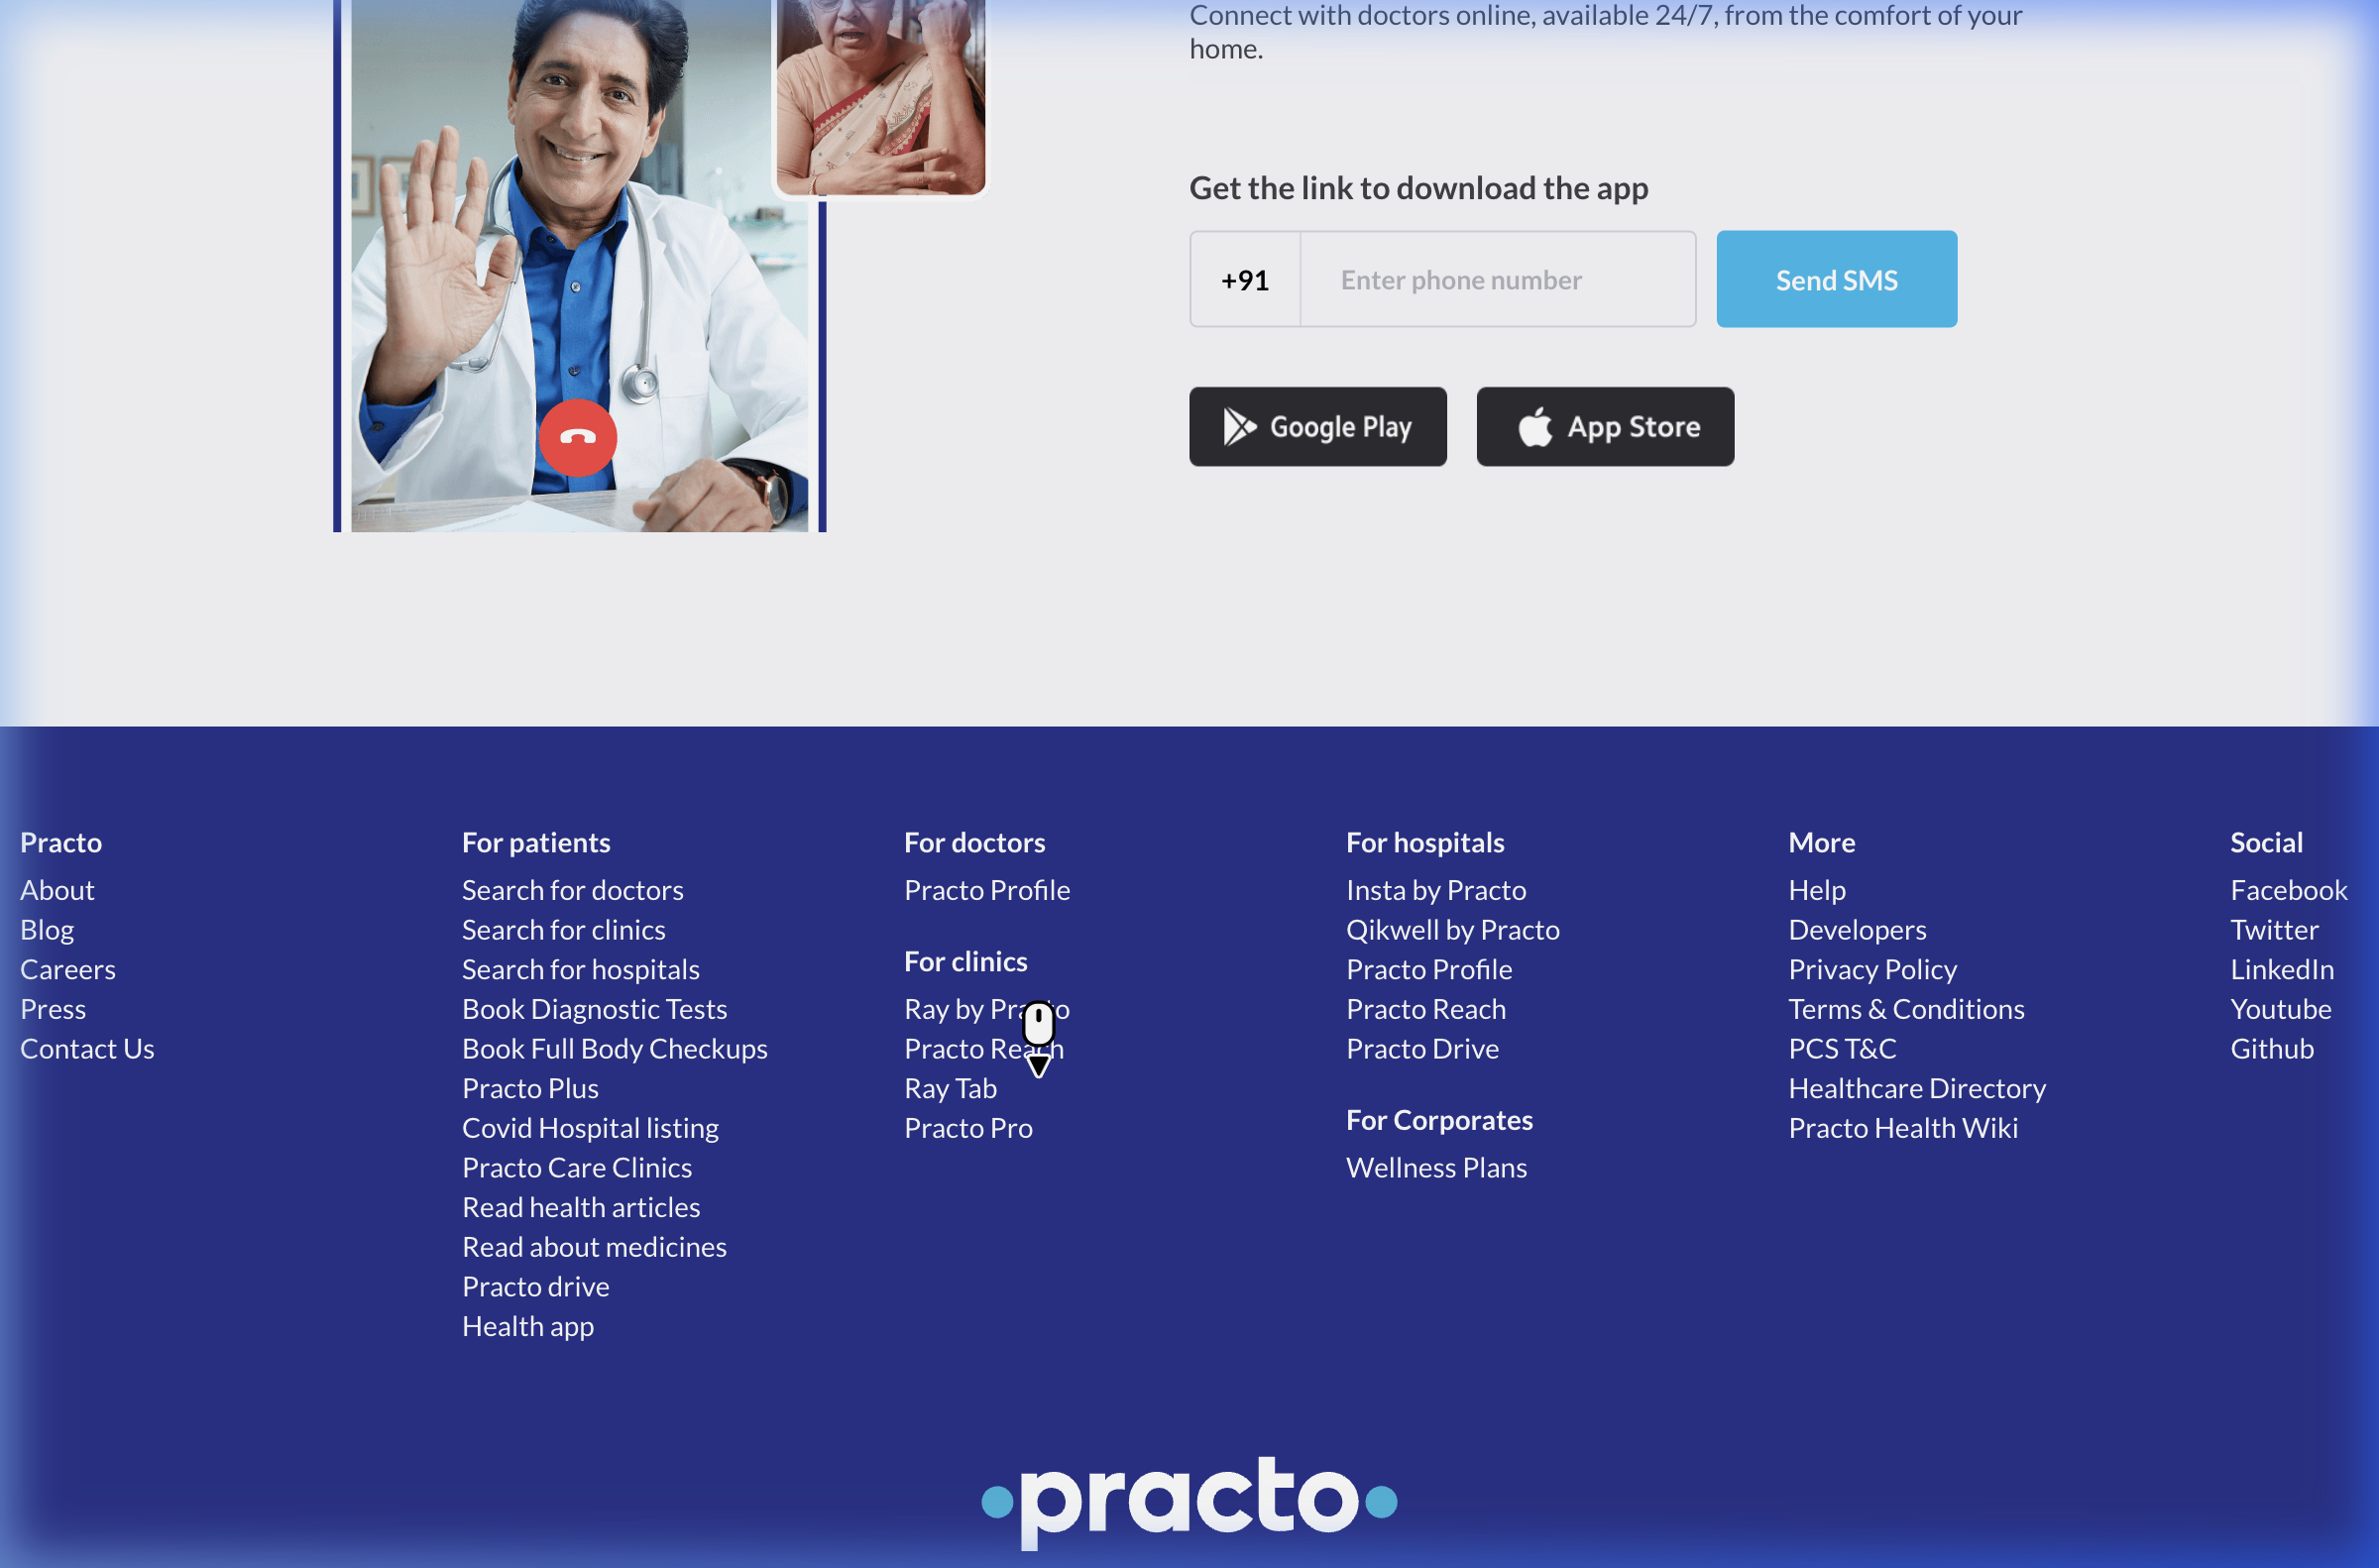
\includegraphics[width=\textwidth]{practo_footer.png}
    \caption{Practo's footer --- 50+ links across 6 columns, overwhelming for users}
\end{figure}

\begin{hcibox}{Miller's Law (7$\pm$2), Hick's Law, Tesler's Law, Nielsen \#8 (Aesthetic Minimalism)}
\textbf{Miller's Law} states that humans can hold 7$\pm$2 chunks in working memory. 50+ links far exceeds this. \textbf{Hick's Law} states decision time increases logarithmically with choices --- more links means longer decision time. \textbf{Tesler's Law} says complexity should be absorbed by the system, not the user. \textbf{Nielsen \#8} calls for aesthetic and minimalist design --- every extra link competes with relevant information.
\end{hcibox}

\begin{solutionbox}
Our footer uses \textbf{4 collapsible sections} with $\leq$7 items each. On mobile, sections are \textbf{accordion-style} (tap to expand). Total visible links reduced from 50+ to a manageable set, respecting Miller's cognitive limits.
\end{solutionbox}

\textit{Screenshot: See the footer at the bottom of any page in our prototype. Navigate to \texttt{http://localhost:5173} and scroll down.}

% TODO: Replace with actual screenshot
% \begin{figure}[H]
%     \centering
%     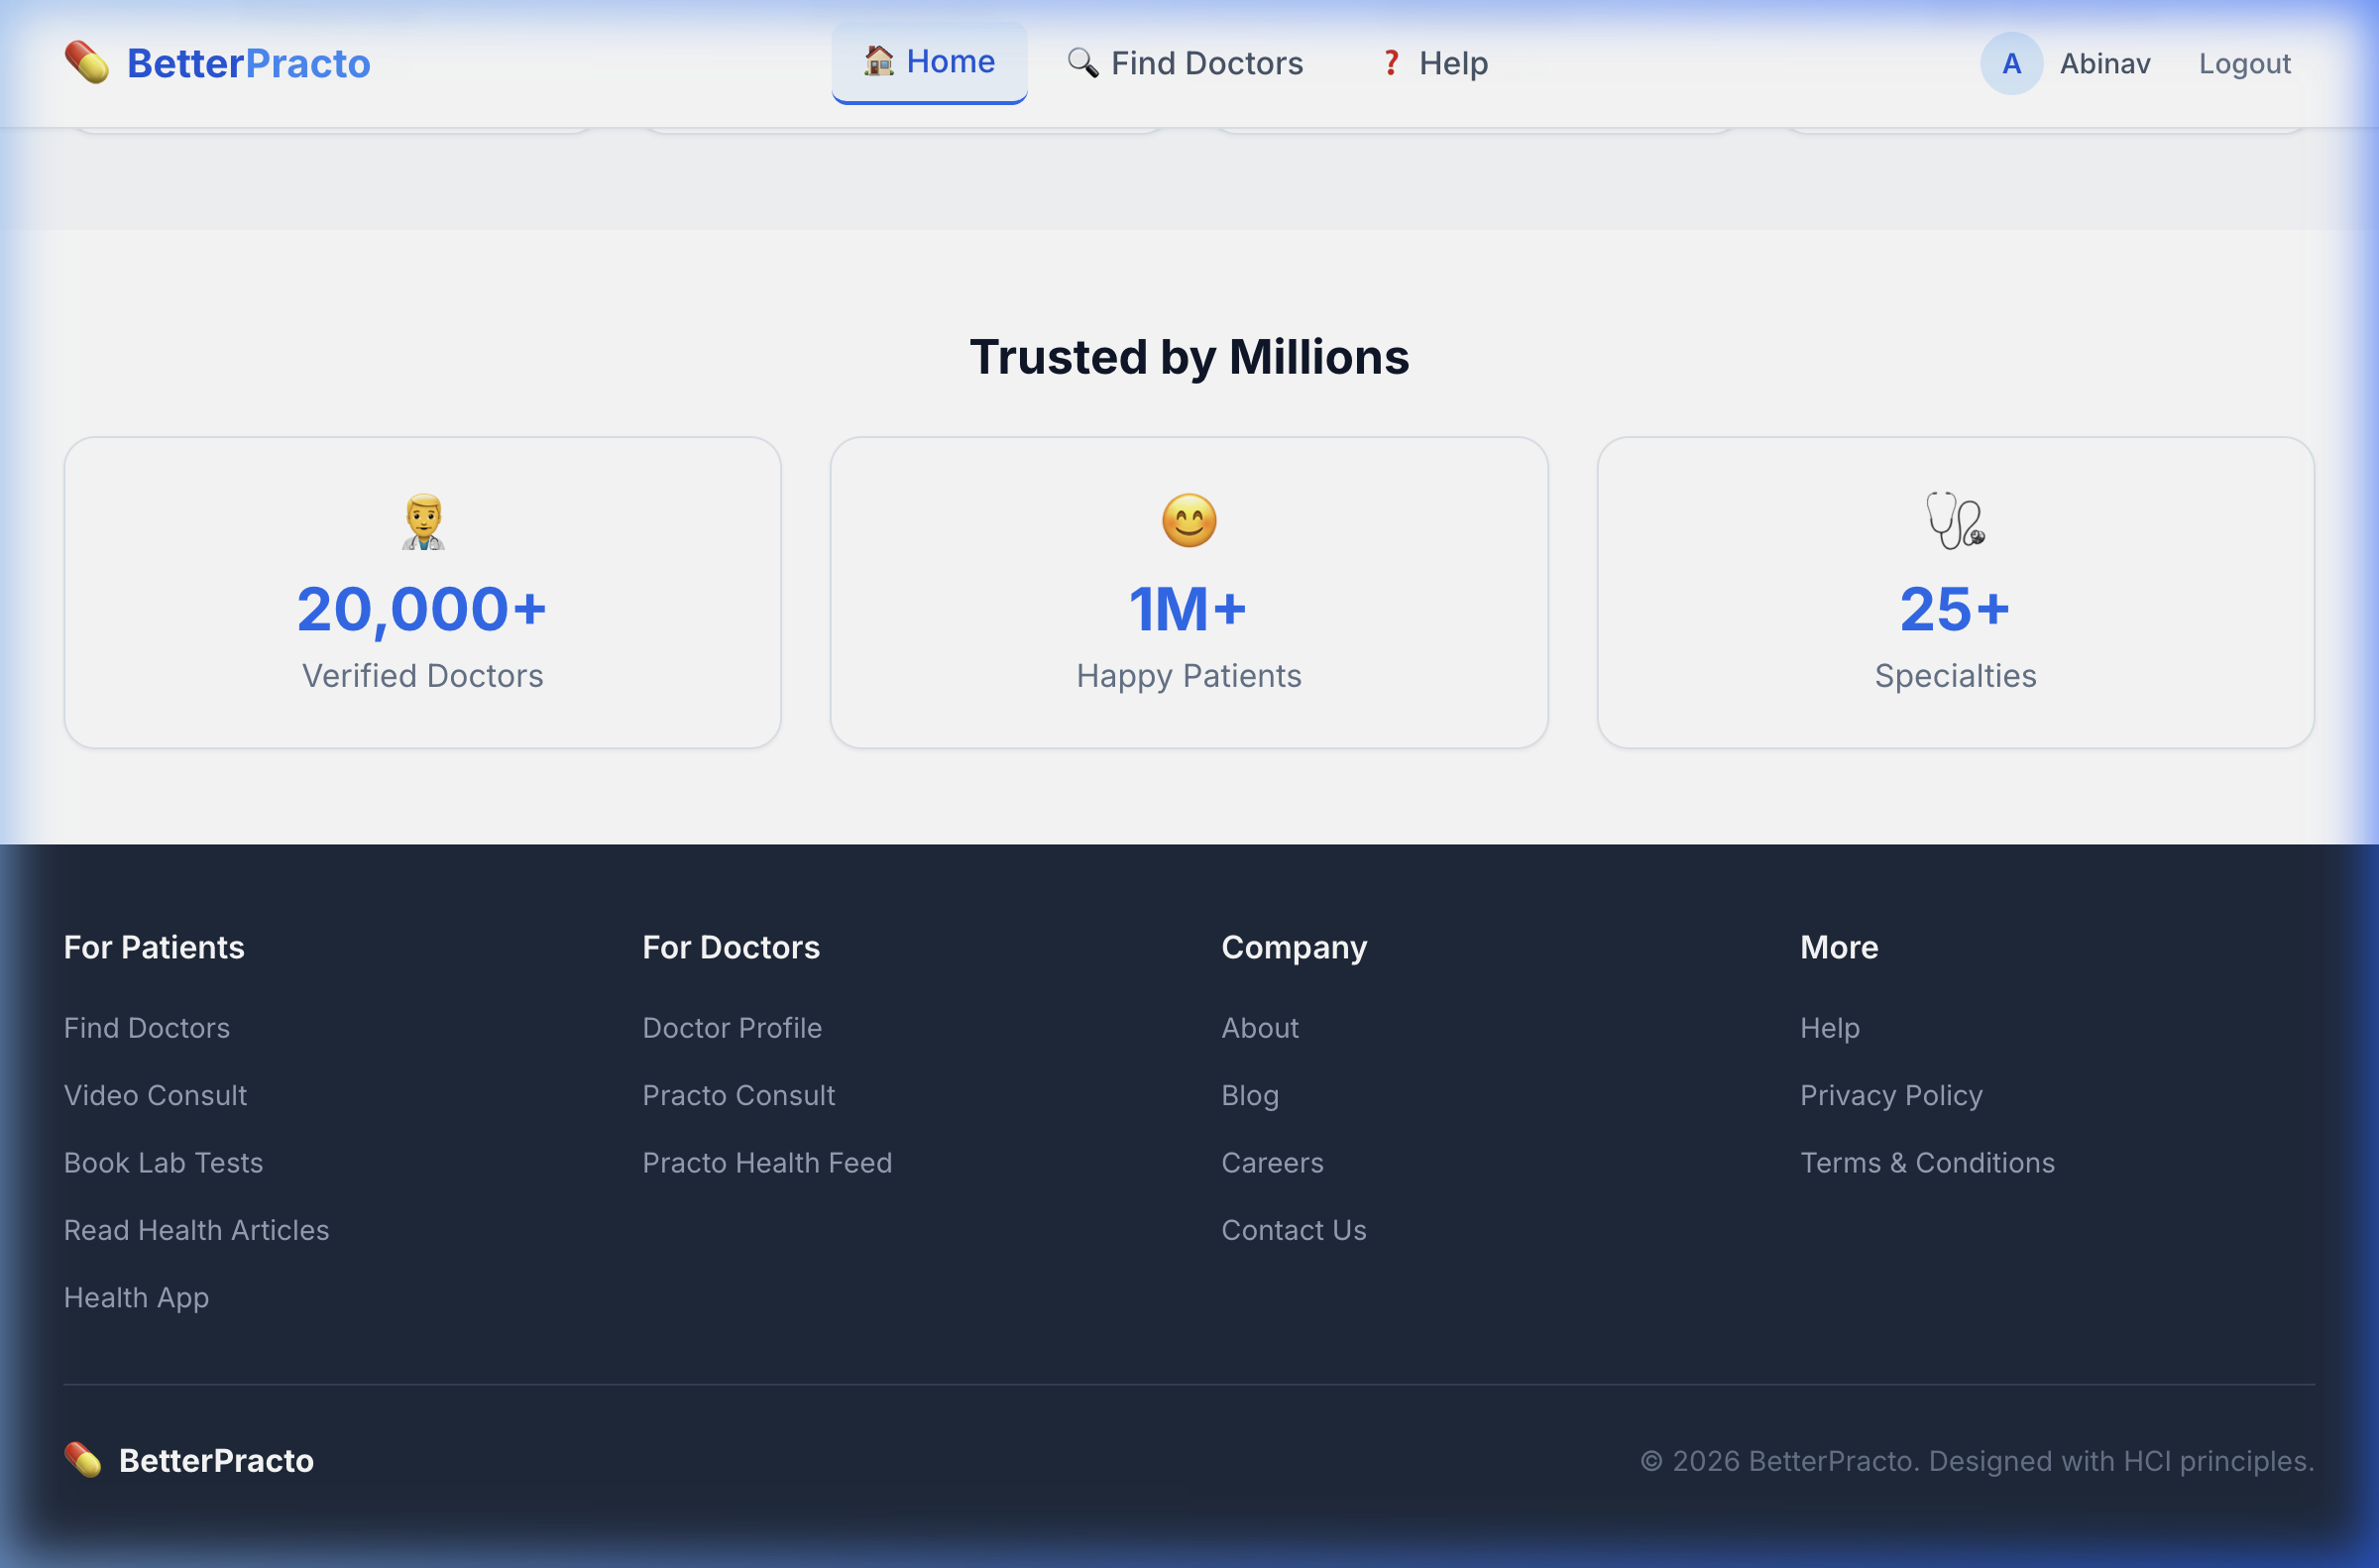
\includegraphics[width=\textwidth]{our_footer.png}
%     \caption{Better Practo --- Clean footer with 4 collapsible sections, $\leq$7 items each}
% \end{figure}

\newpage

% ----------------------------------------------------------------
\subsection{V2: Dual Search Bar (Location + Query)}

\begin{violationbox}
Practo's homepage features \textbf{two separate search inputs} side-by-side: one for location (``Search location'') and one for the query (``Search doctors, clinics, hospitals, etc.''). The user must interact with both fields before searching, adding unnecessary cognitive load and effort.
\end{violationbox}

\begin{figure}[H]
    \centering
    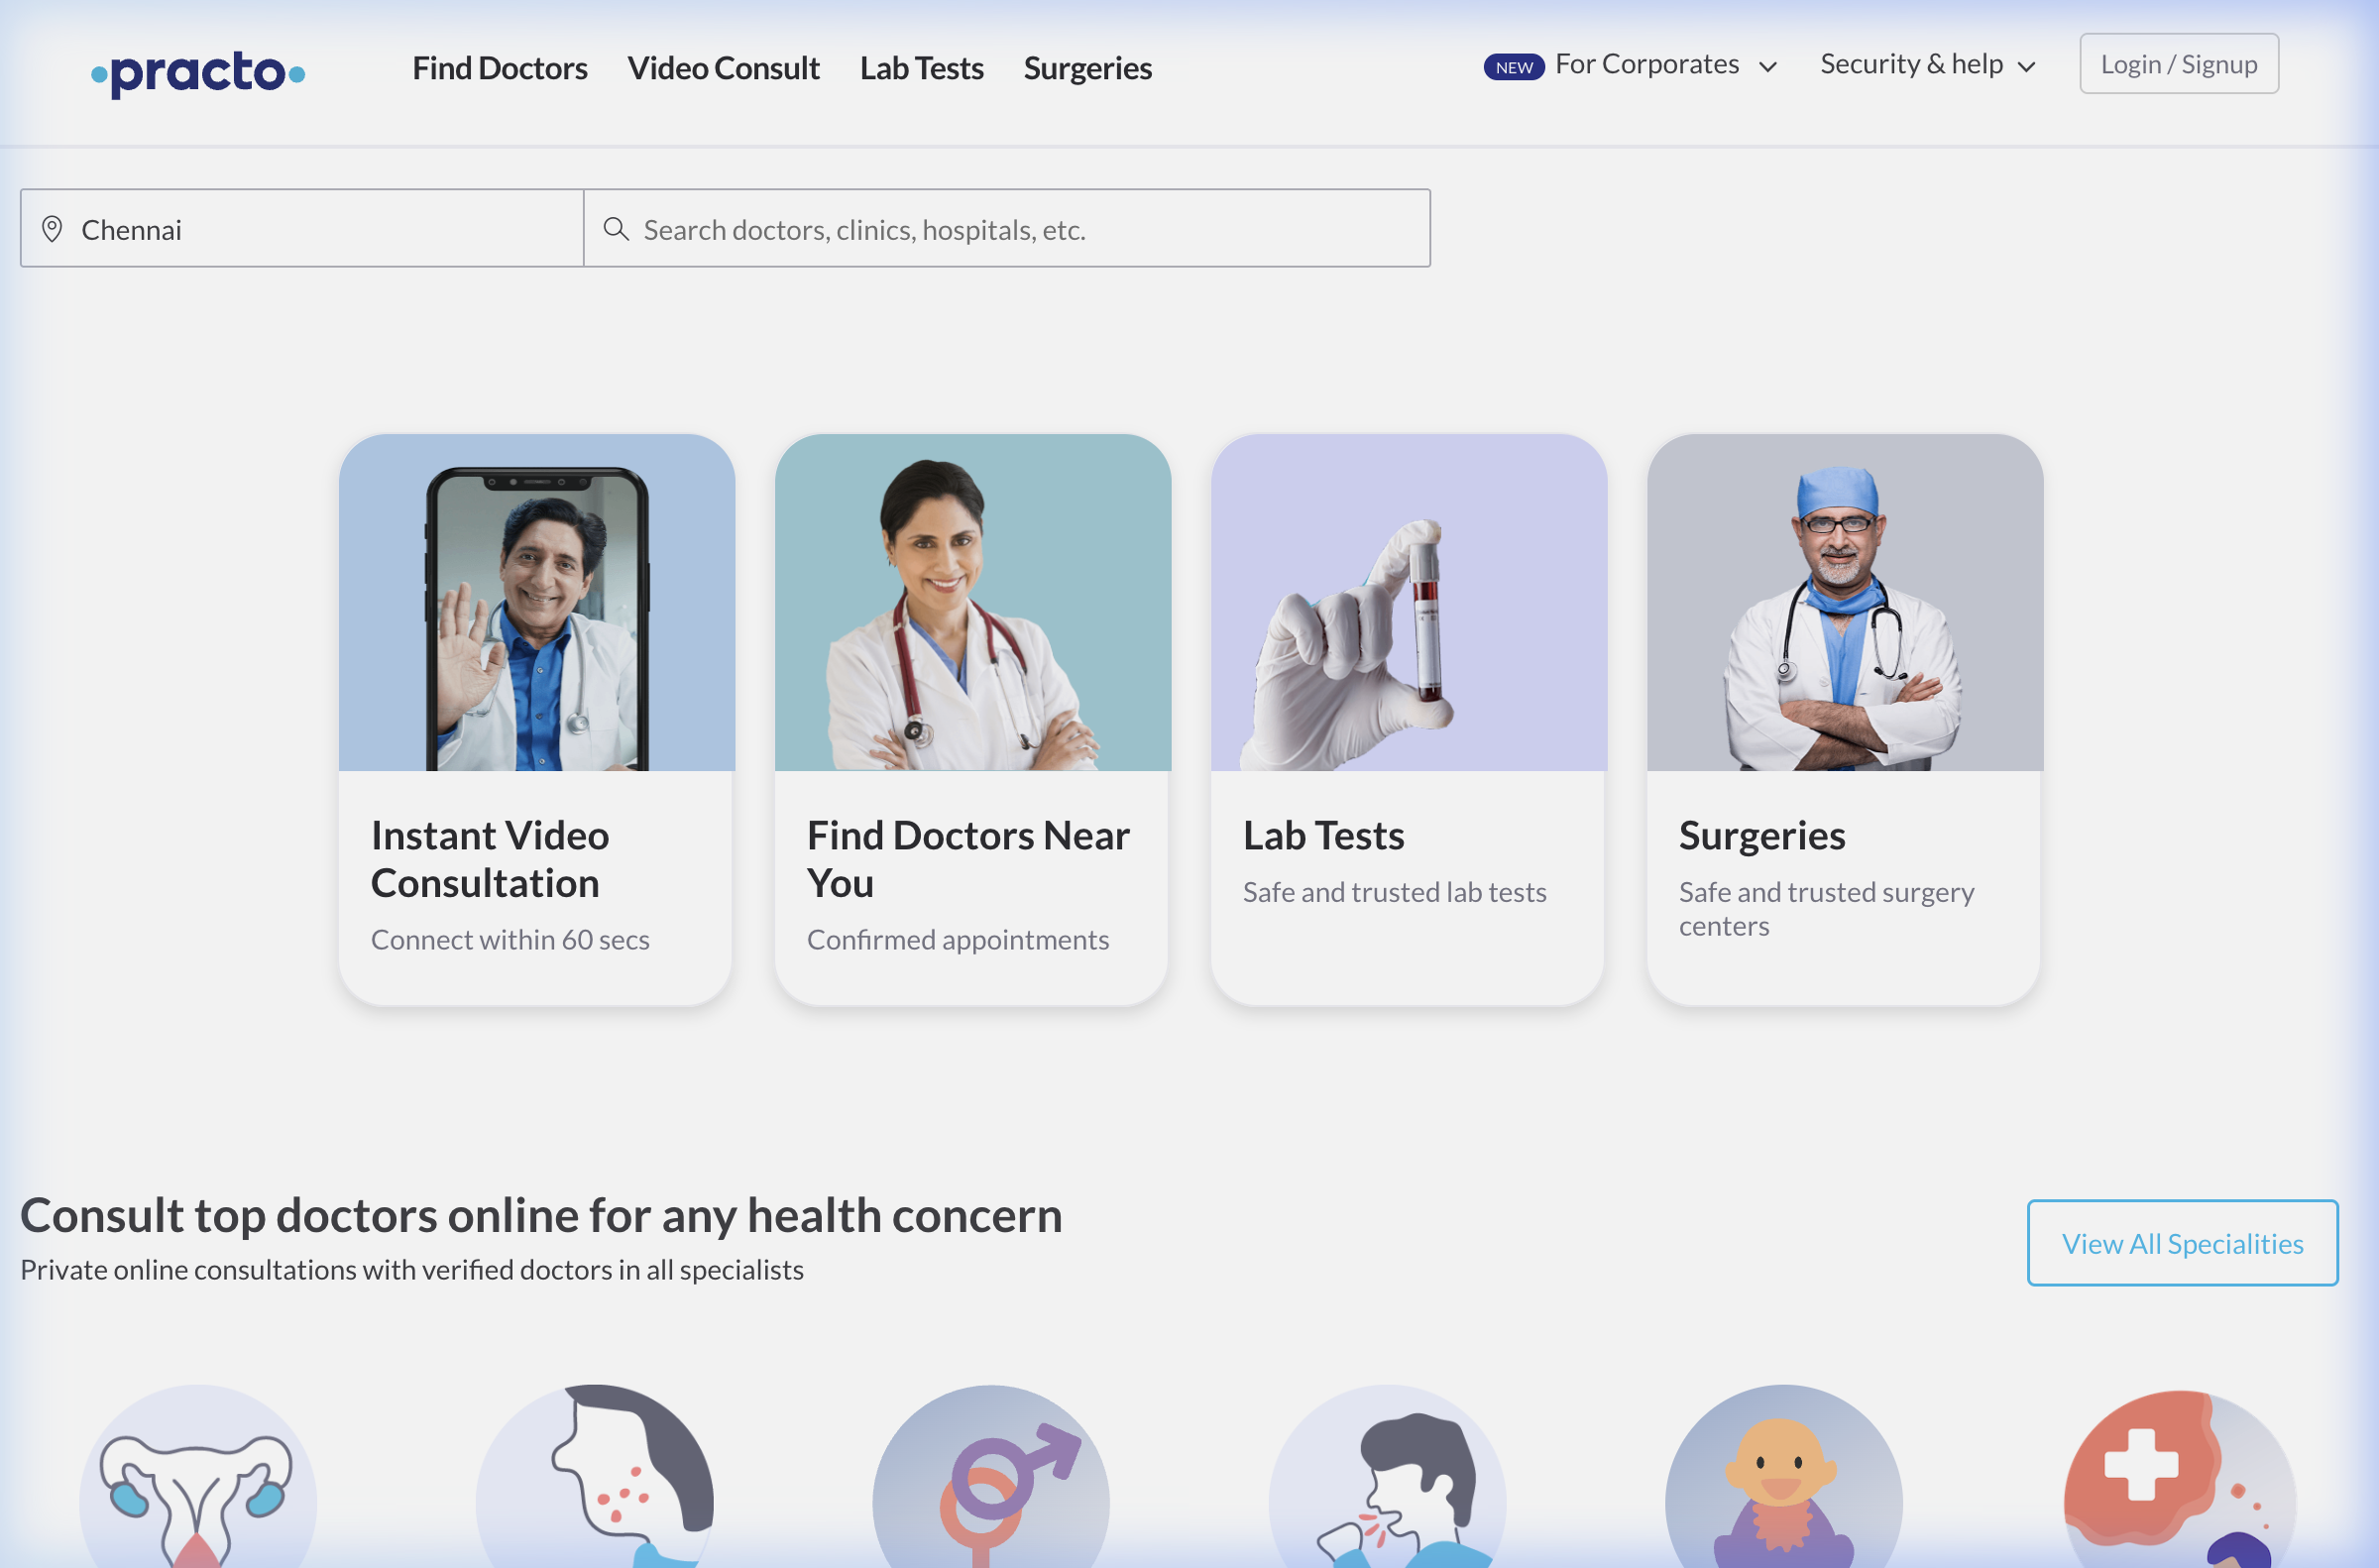
\includegraphics[width=\textwidth]{practo_homepage.png}
    \caption{Practo's dual search bar --- two separate inputs for location and query}
\end{figure}

\begin{hcibox}{Tesler's Law, Zipf's Law (Least Effort), Asimov's 2nd Law}
\textbf{Tesler's Law} (Conservation of Complexity) says the system should absorb complexity --- auto-detecting location is trivially doable. \textbf{Zipf's Law} says users follow the path of least effort --- forcing two inputs when one suffices adds unnecessary friction. \textbf{Asimov's 2nd Law} (Don't waste the user's time) --- if the system can detect location, it should.
\end{hcibox}

\begin{solutionbox}
We provide a \textbf{single unified search bar} where users type doctor names, specialties, or symptoms. Location is \textbf{auto-detected} and displayed as a small chip (``$\mathcircled{}$ Chennai'') that can be changed with a tap. One input, zero friction.
\end{solutionbox}

% TODO: Replace with actual screenshot
% \begin{figure}[H]
%     \centering
%     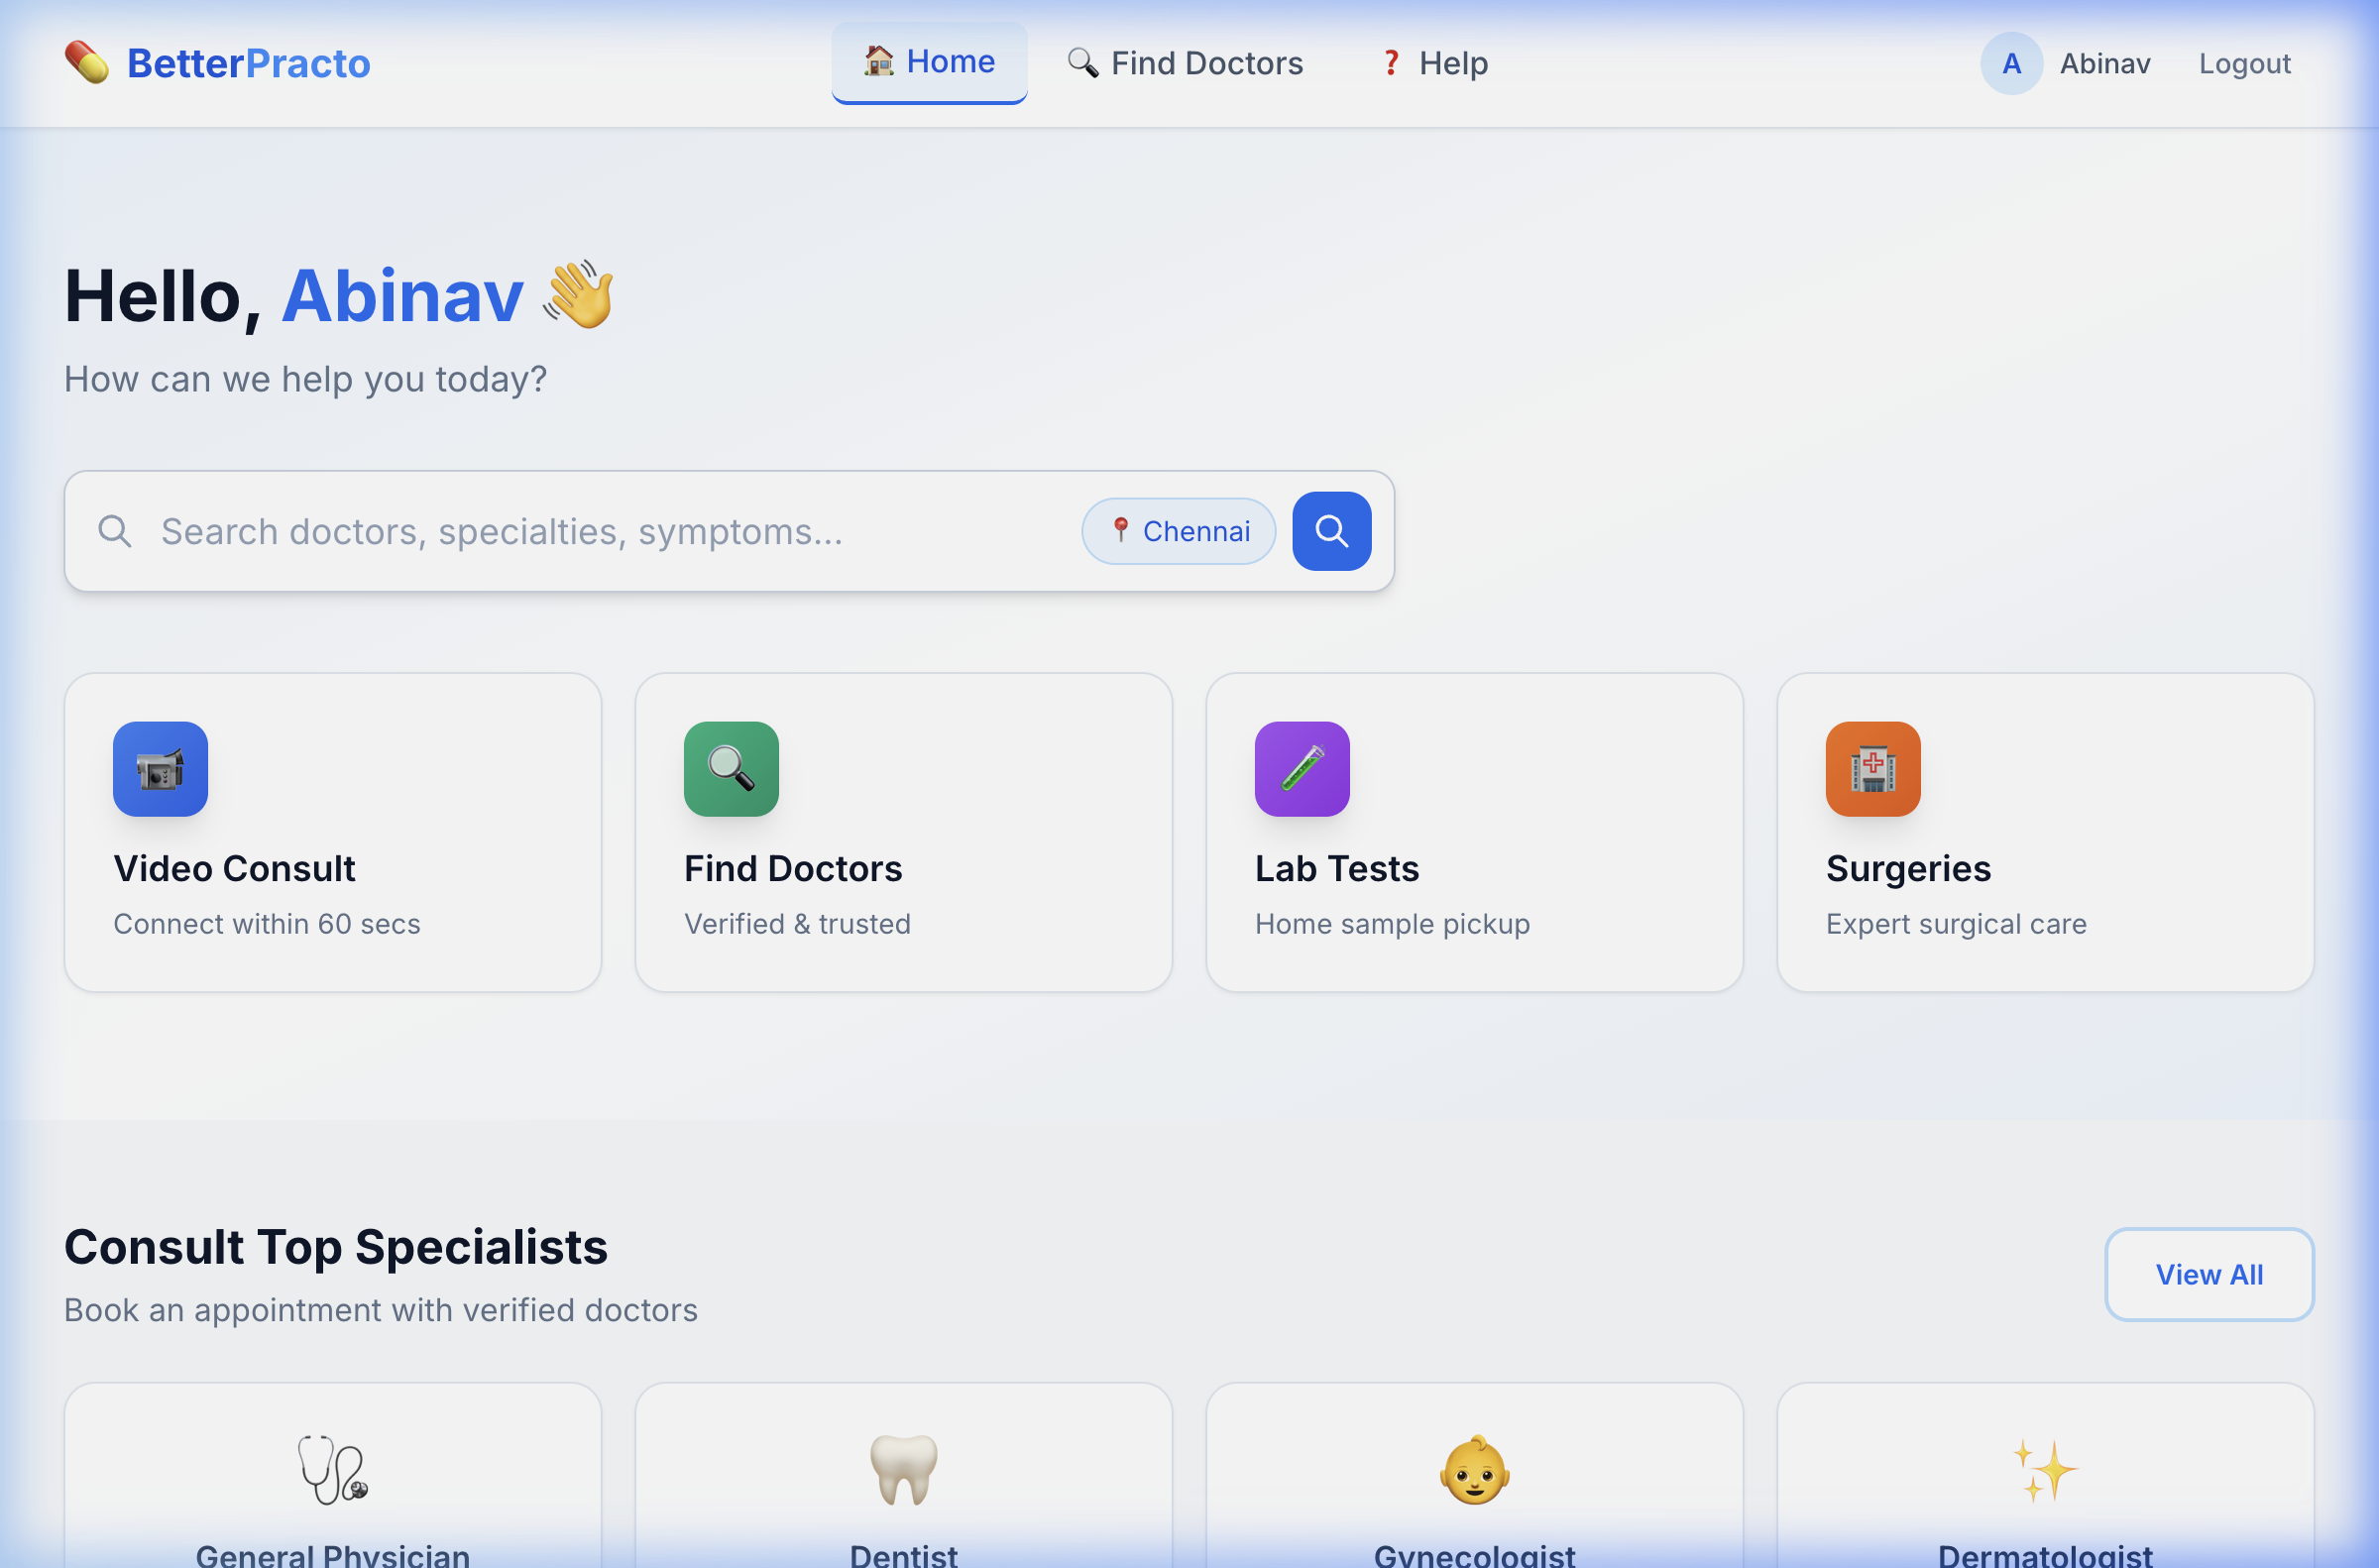
\includegraphics[width=\textwidth]{our_home.png}
%     \caption{Better Practo --- Unified search with auto-detected location chip}
% \end{figure}

\newpage

% ----------------------------------------------------------------
\subsection{V3: Cluttered Doctor Cards}

\begin{violationbox}
Practo's doctor search results show \textbf{everything at once} on each card: name, specialty, experience, location, hospital, consultation fee, rating percentage, patient story count, badges (``Practo Dental''), availability, and two CTAs (``Book Clinic Visit'' + ``Contact Clinic''). This creates information overload and makes it hard to compare doctors efficiently.
\end{violationbox}

\begin{figure}[H]
    \centering
    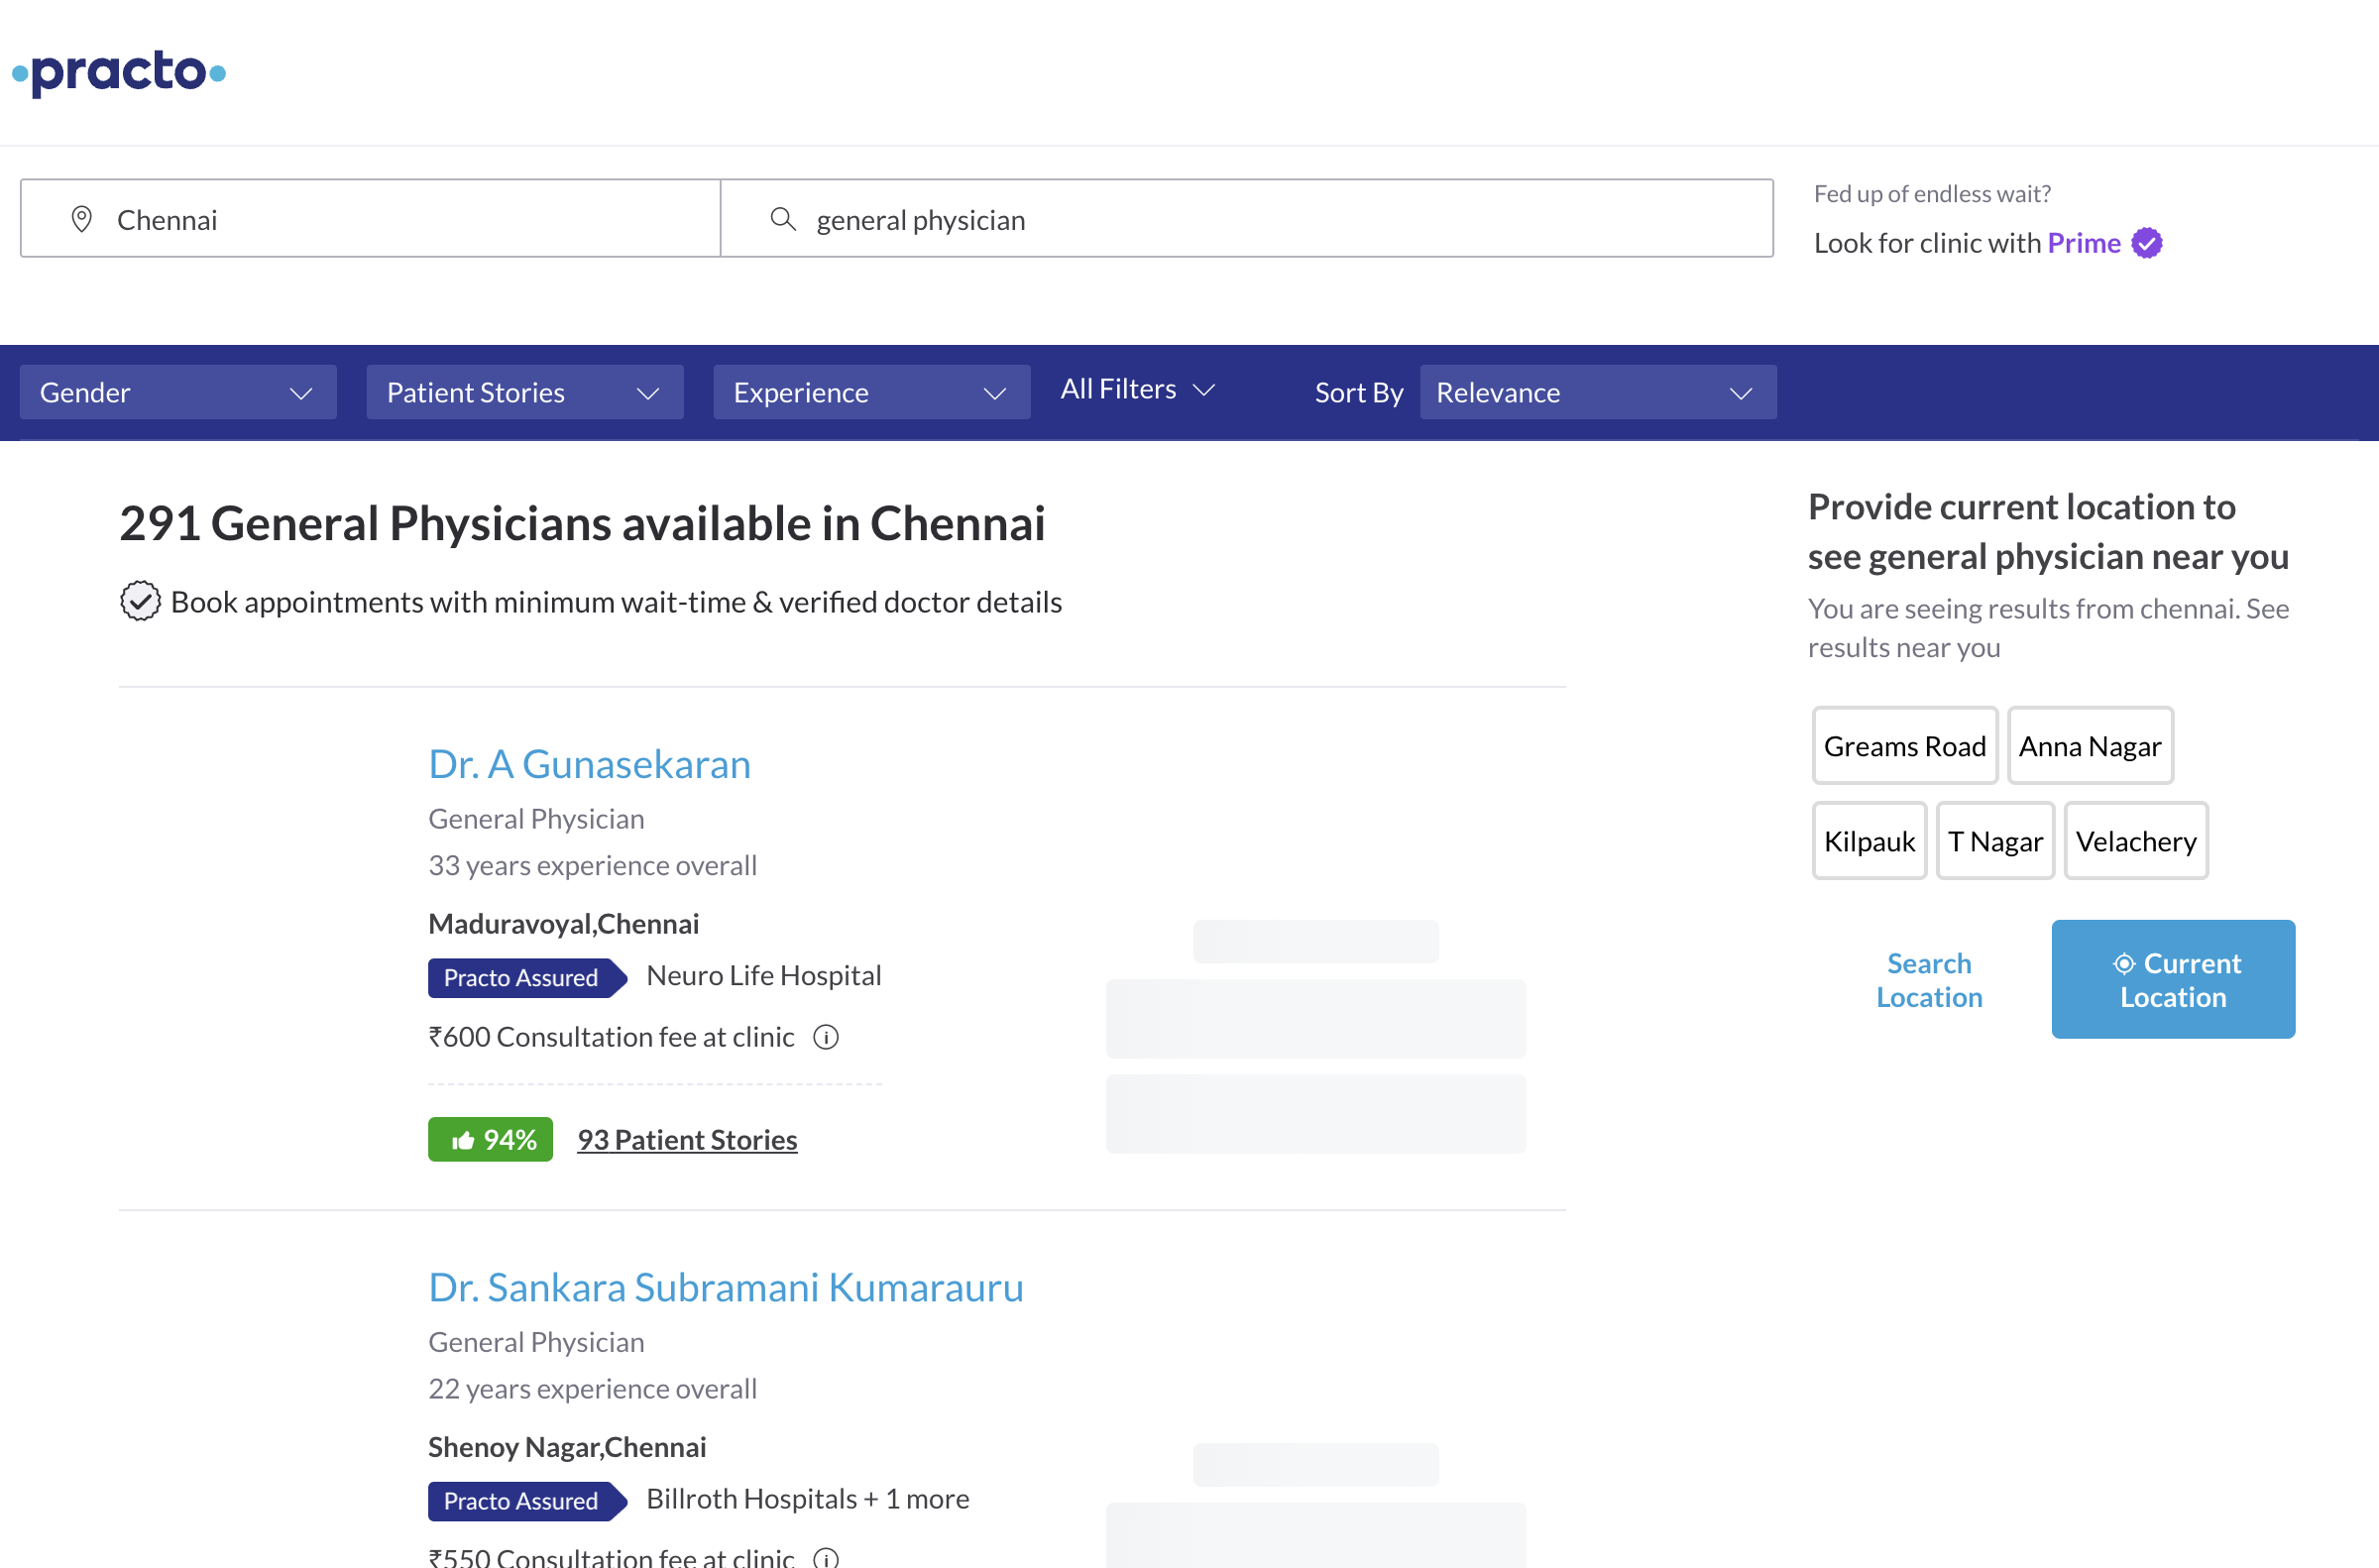
\includegraphics[width=\textwidth]{practo_search_results.png}
    \caption{Practo's search results --- dense doctor cards with too much information at once}
\end{figure}

\begin{hcibox}{Inverted Pyramid, Nielsen \#8 (Aesthetic Minimalism), Progressive Disclosure}
The \textbf{Inverted Pyramid} principle says the most important information should come first, with details progressively revealed. \textbf{Nielsen \#8} warns against cluttering the interface with rarely-needed information. \textbf{Progressive Disclosure} means showing only essential info initially and revealing details on demand.
\end{hcibox}

\begin{solutionbox}
Our doctor cards show only \textbf{essential information} upfront: name, specialty, rating, and availability. Additional details (education, hospital, about) are hidden behind a \textbf{``More details''} expand button. This applies tighter progressive disclosure with a cleaner information hierarchy.
\end{solutionbox}

\begin{figure}[H]
    \centering
    \begin{subfigure}[b]{0.48\textwidth}
        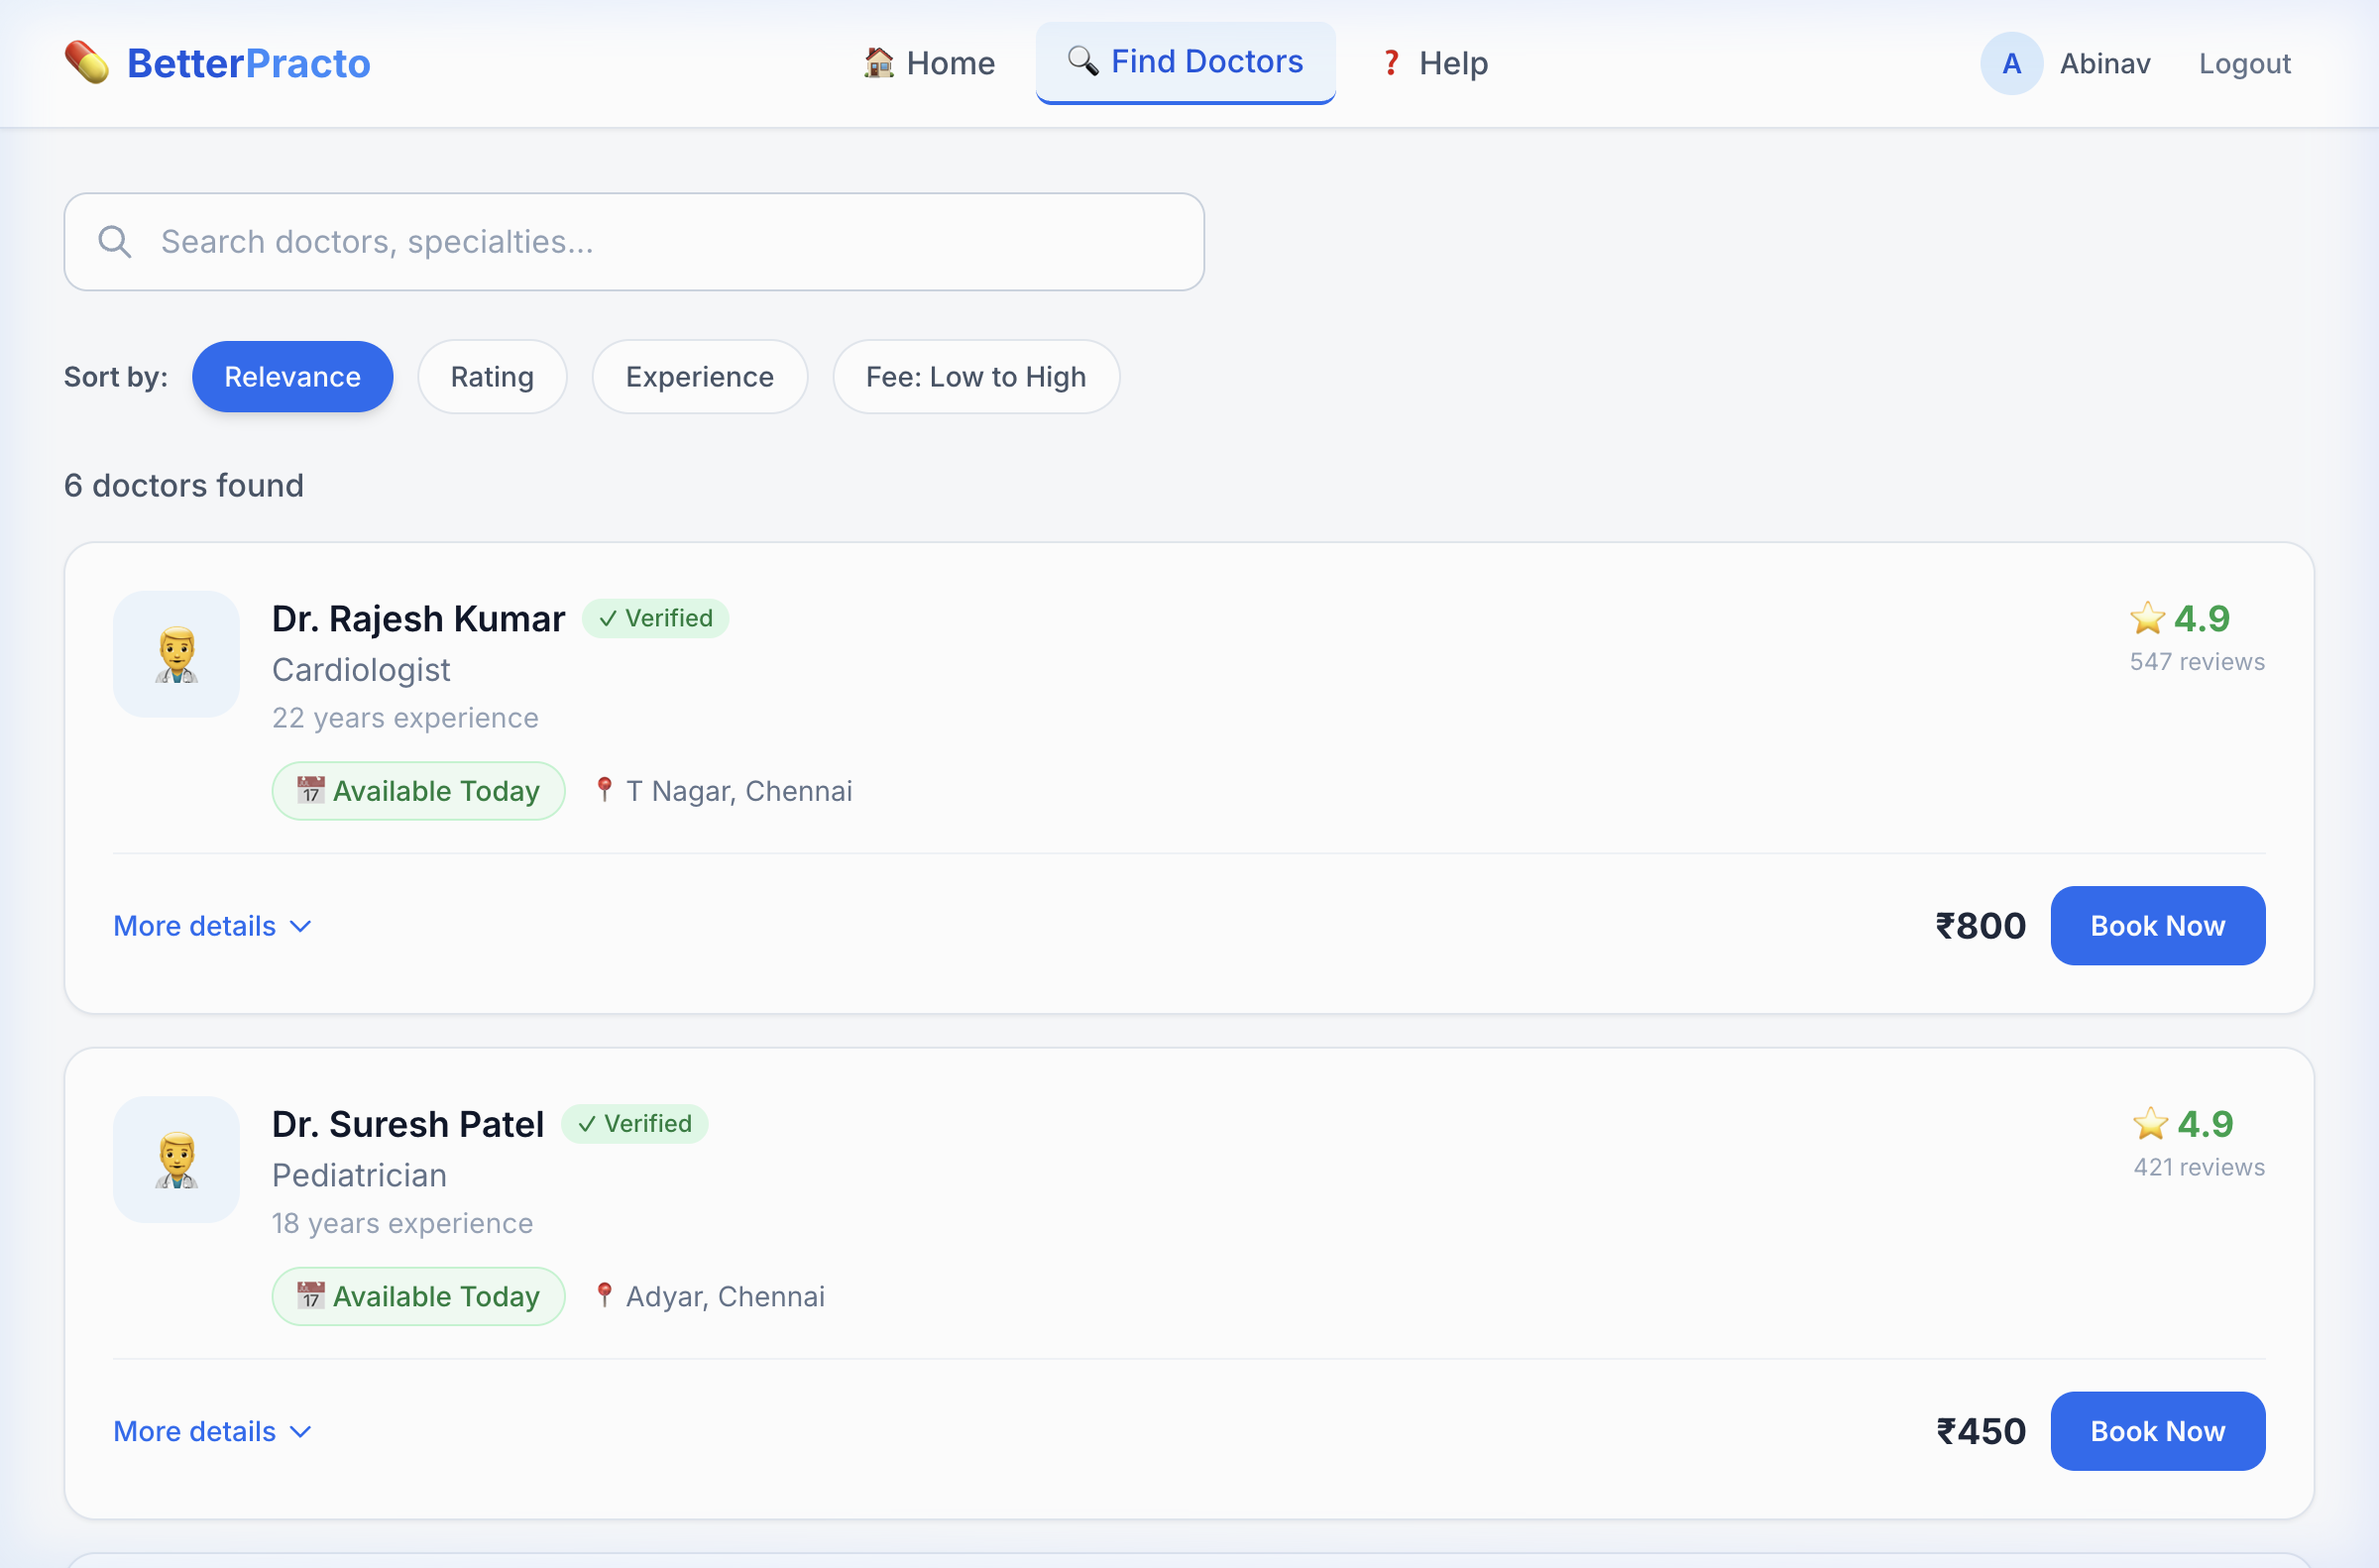
\includegraphics[width=\textwidth]{our_search_results.png}
        \caption{Collapsed cards --- essentials only}
    \end{subfigure}
    \hfill
    \begin{subfigure}[b]{0.48\textwidth}
        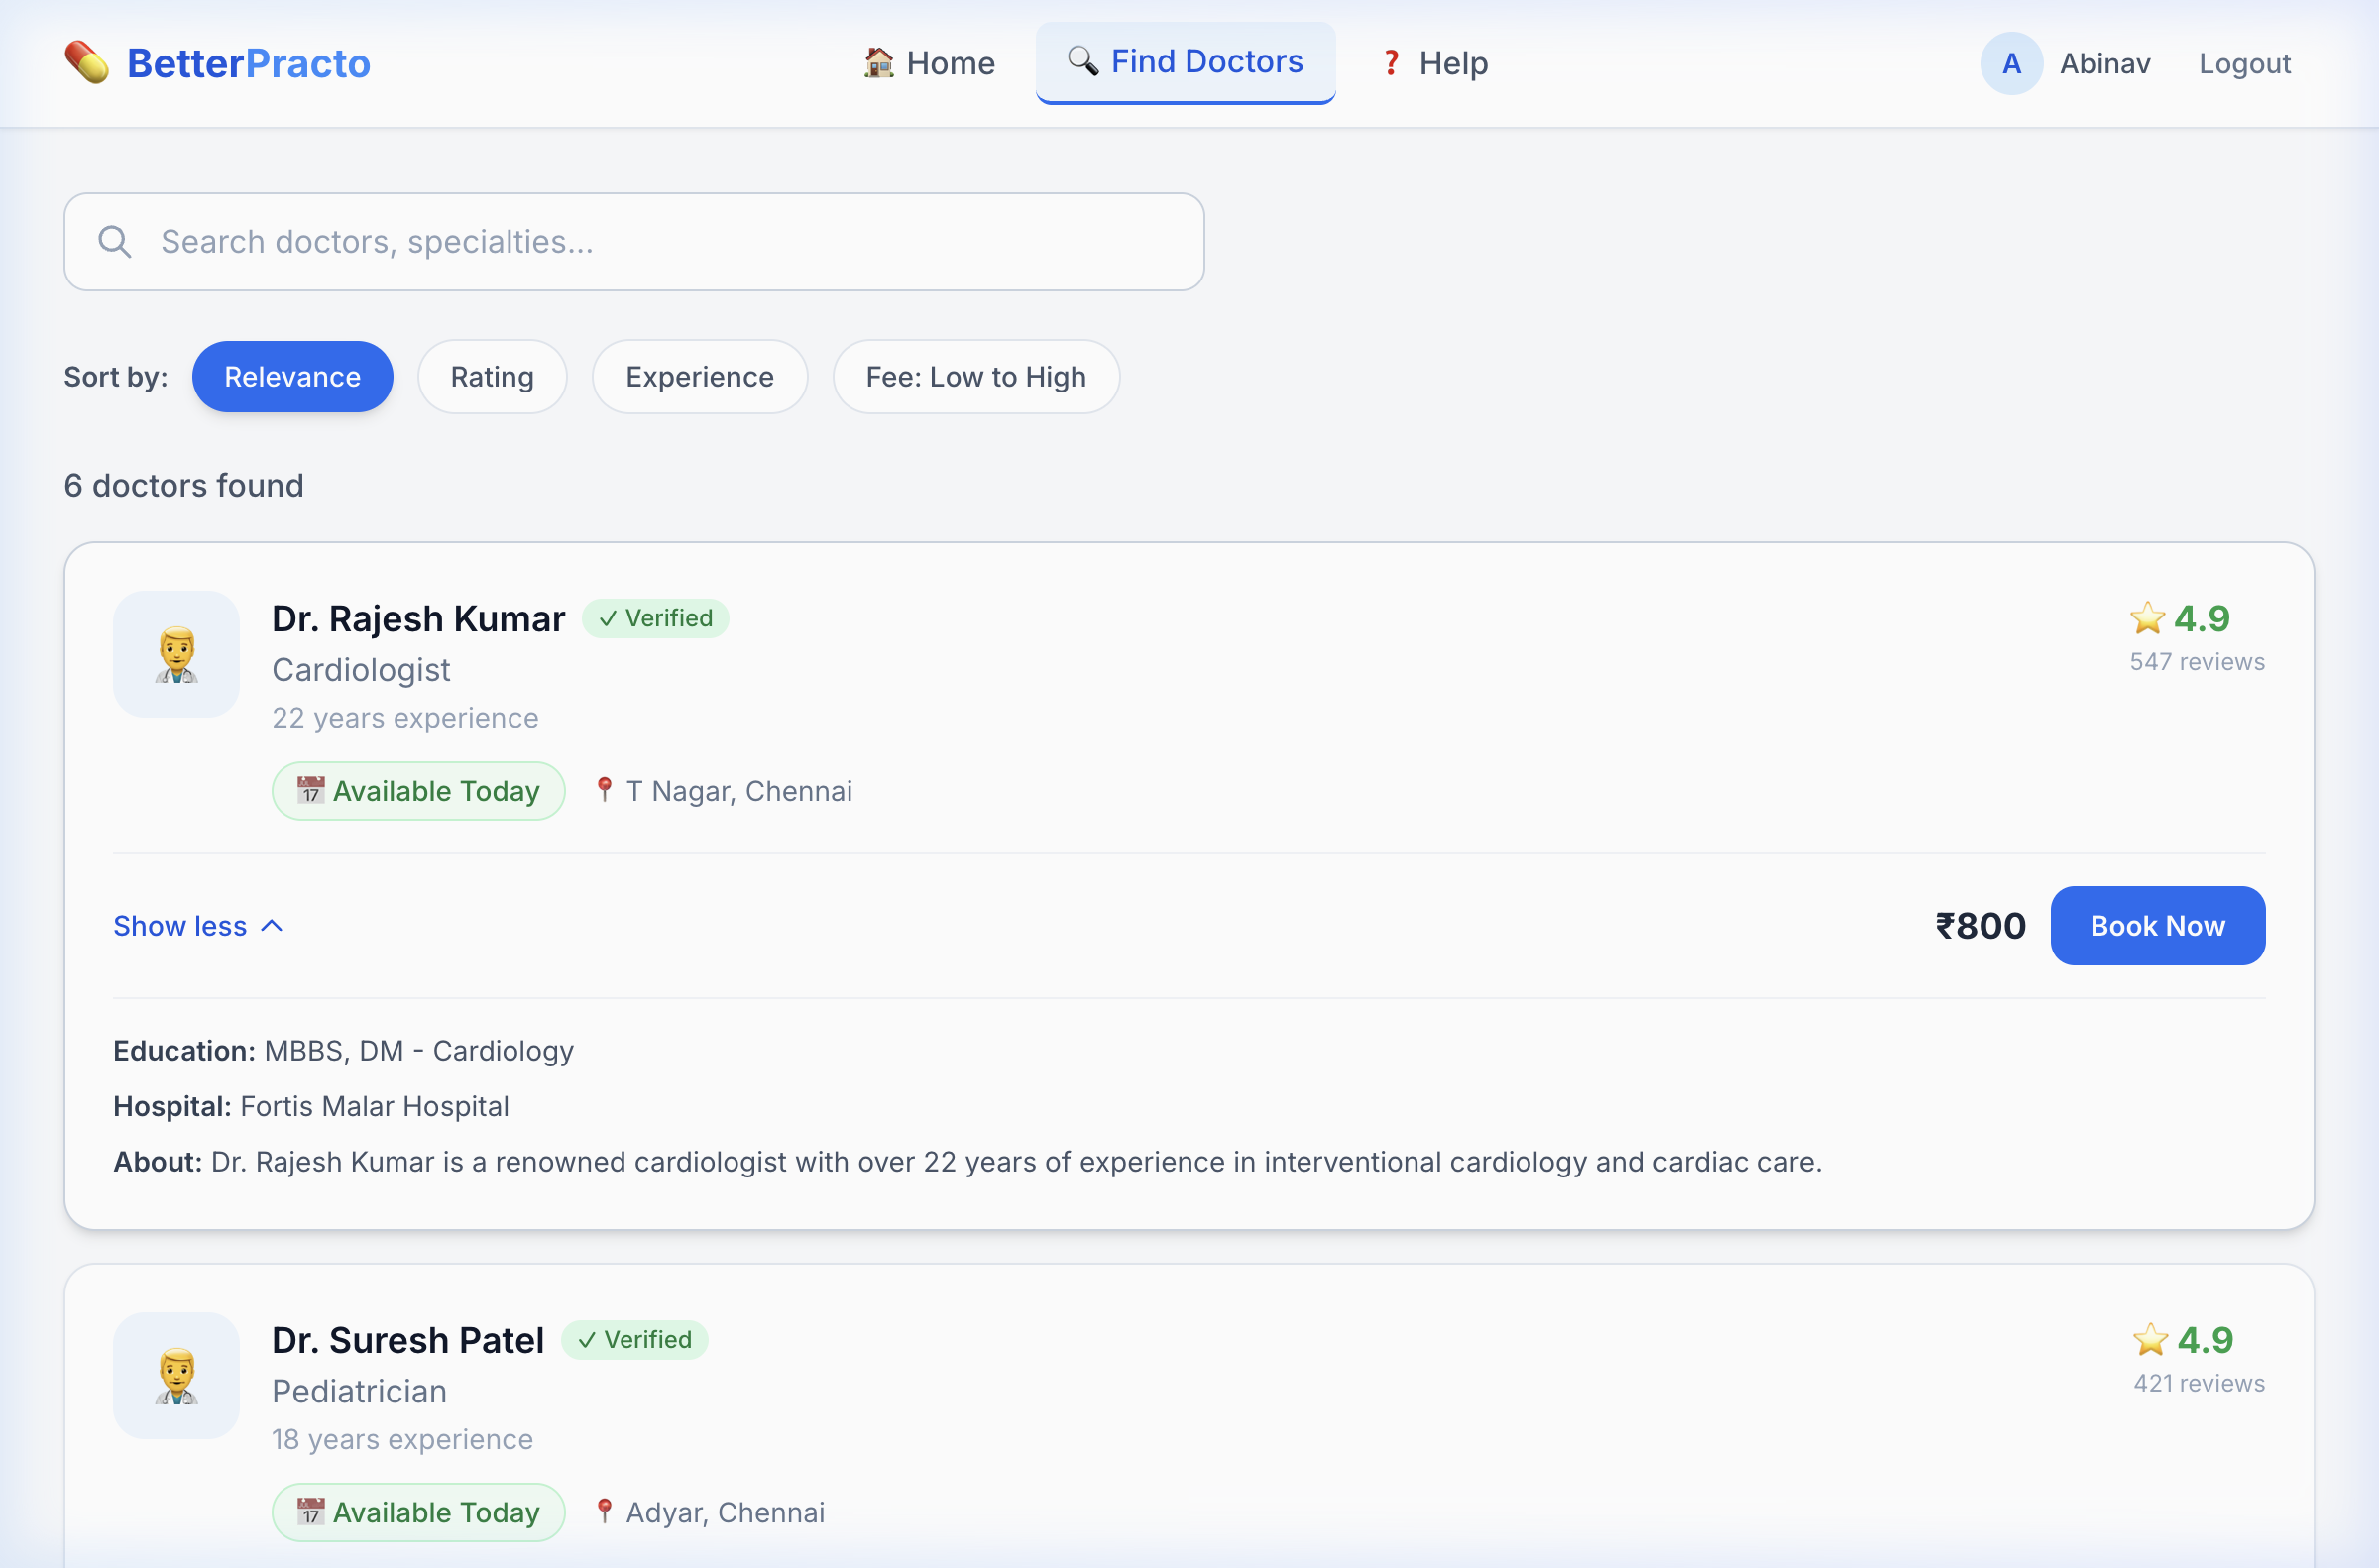
\includegraphics[width=\textwidth]{our_expanded_card.png}
        \caption{Expanded --- full details on demand}
    \end{subfigure}
    \caption{Better Practo --- Progressive disclosure on doctor cards}
\end{figure}

\newpage

% ----------------------------------------------------------------
\subsection{V5 + V14: Weak Booking Feedback \& No Progress Indicator}

\begin{violationbox}
Practo's booking flow has \textbf{no progress indicator} --- the user doesn't know how many steps remain or where they are in the process. The ``Continue'' button is greyed out with no explanation. After confirming, there is no meaningful success feedback. The only navigation option is ``Go back to my results'' --- poor user control.
\end{violationbox}

\begin{figure}[H]
    \centering
    \begin{subfigure}[b]{0.48\textwidth}
        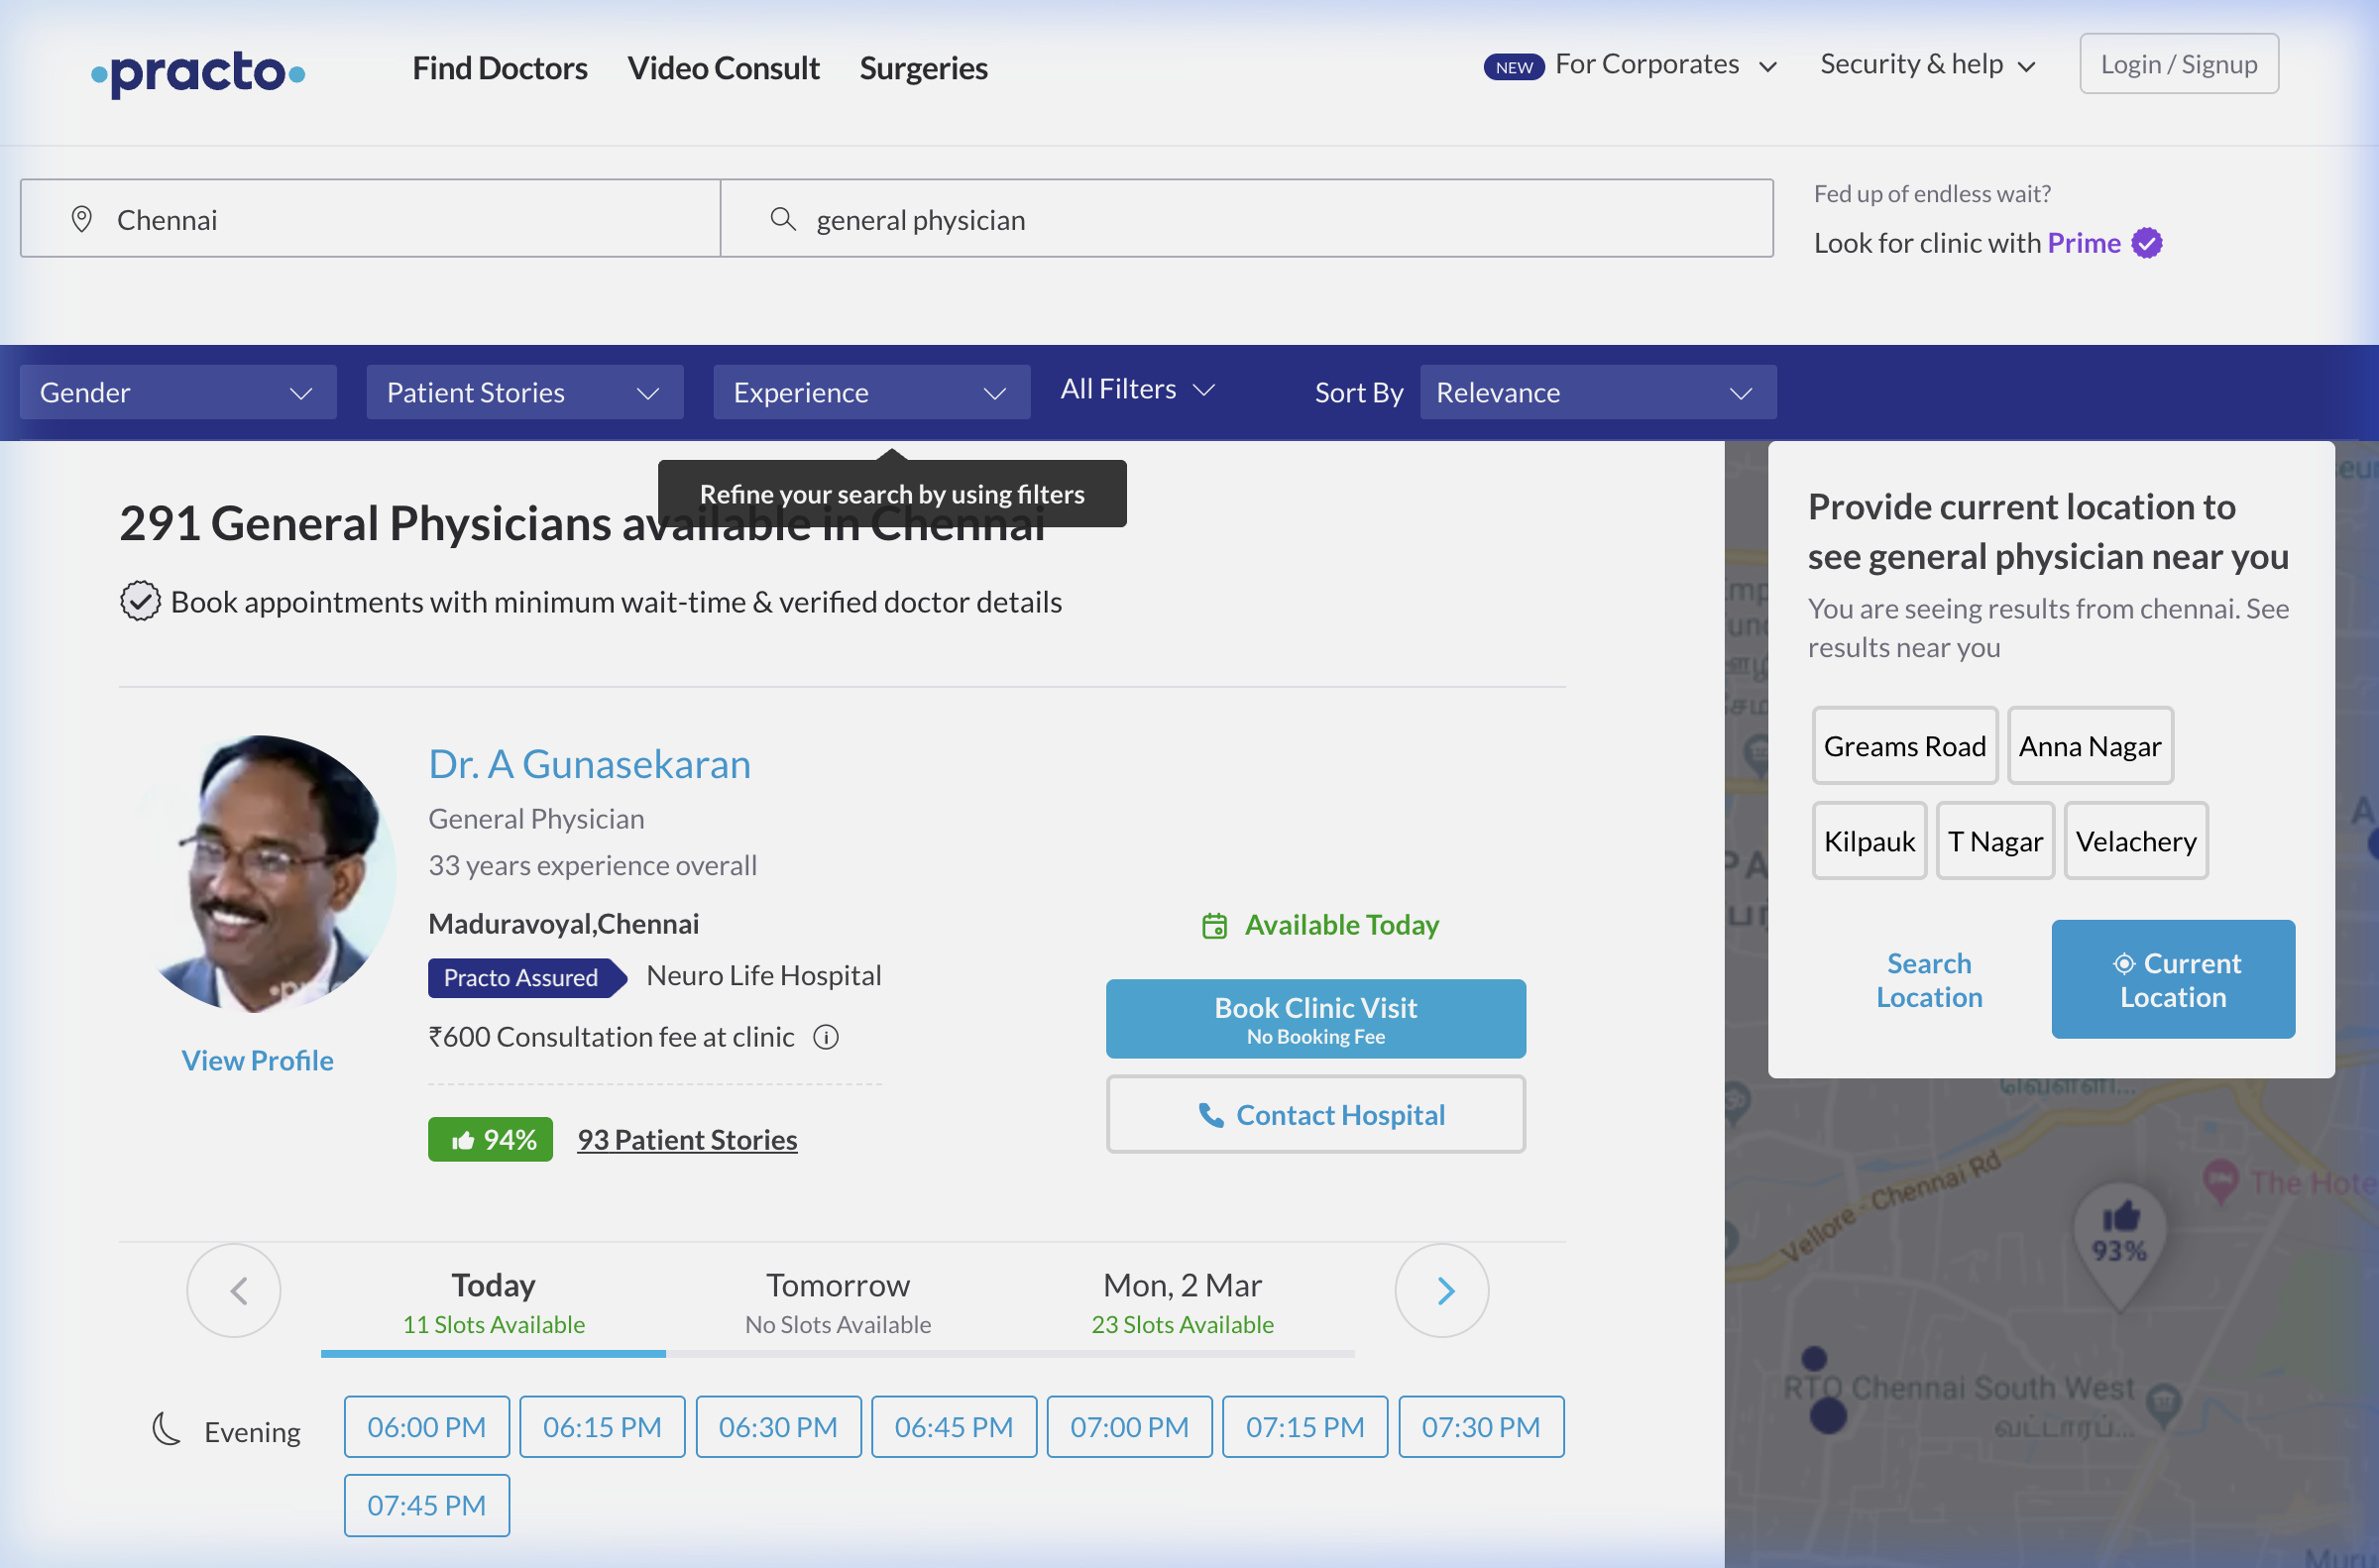
\includegraphics[width=\textwidth]{practo_booking_slots.png}
        \caption{Slot selection --- no progress bar}
    \end{subfigure}
    \hfill
    \begin{subfigure}[b]{0.48\textwidth}
        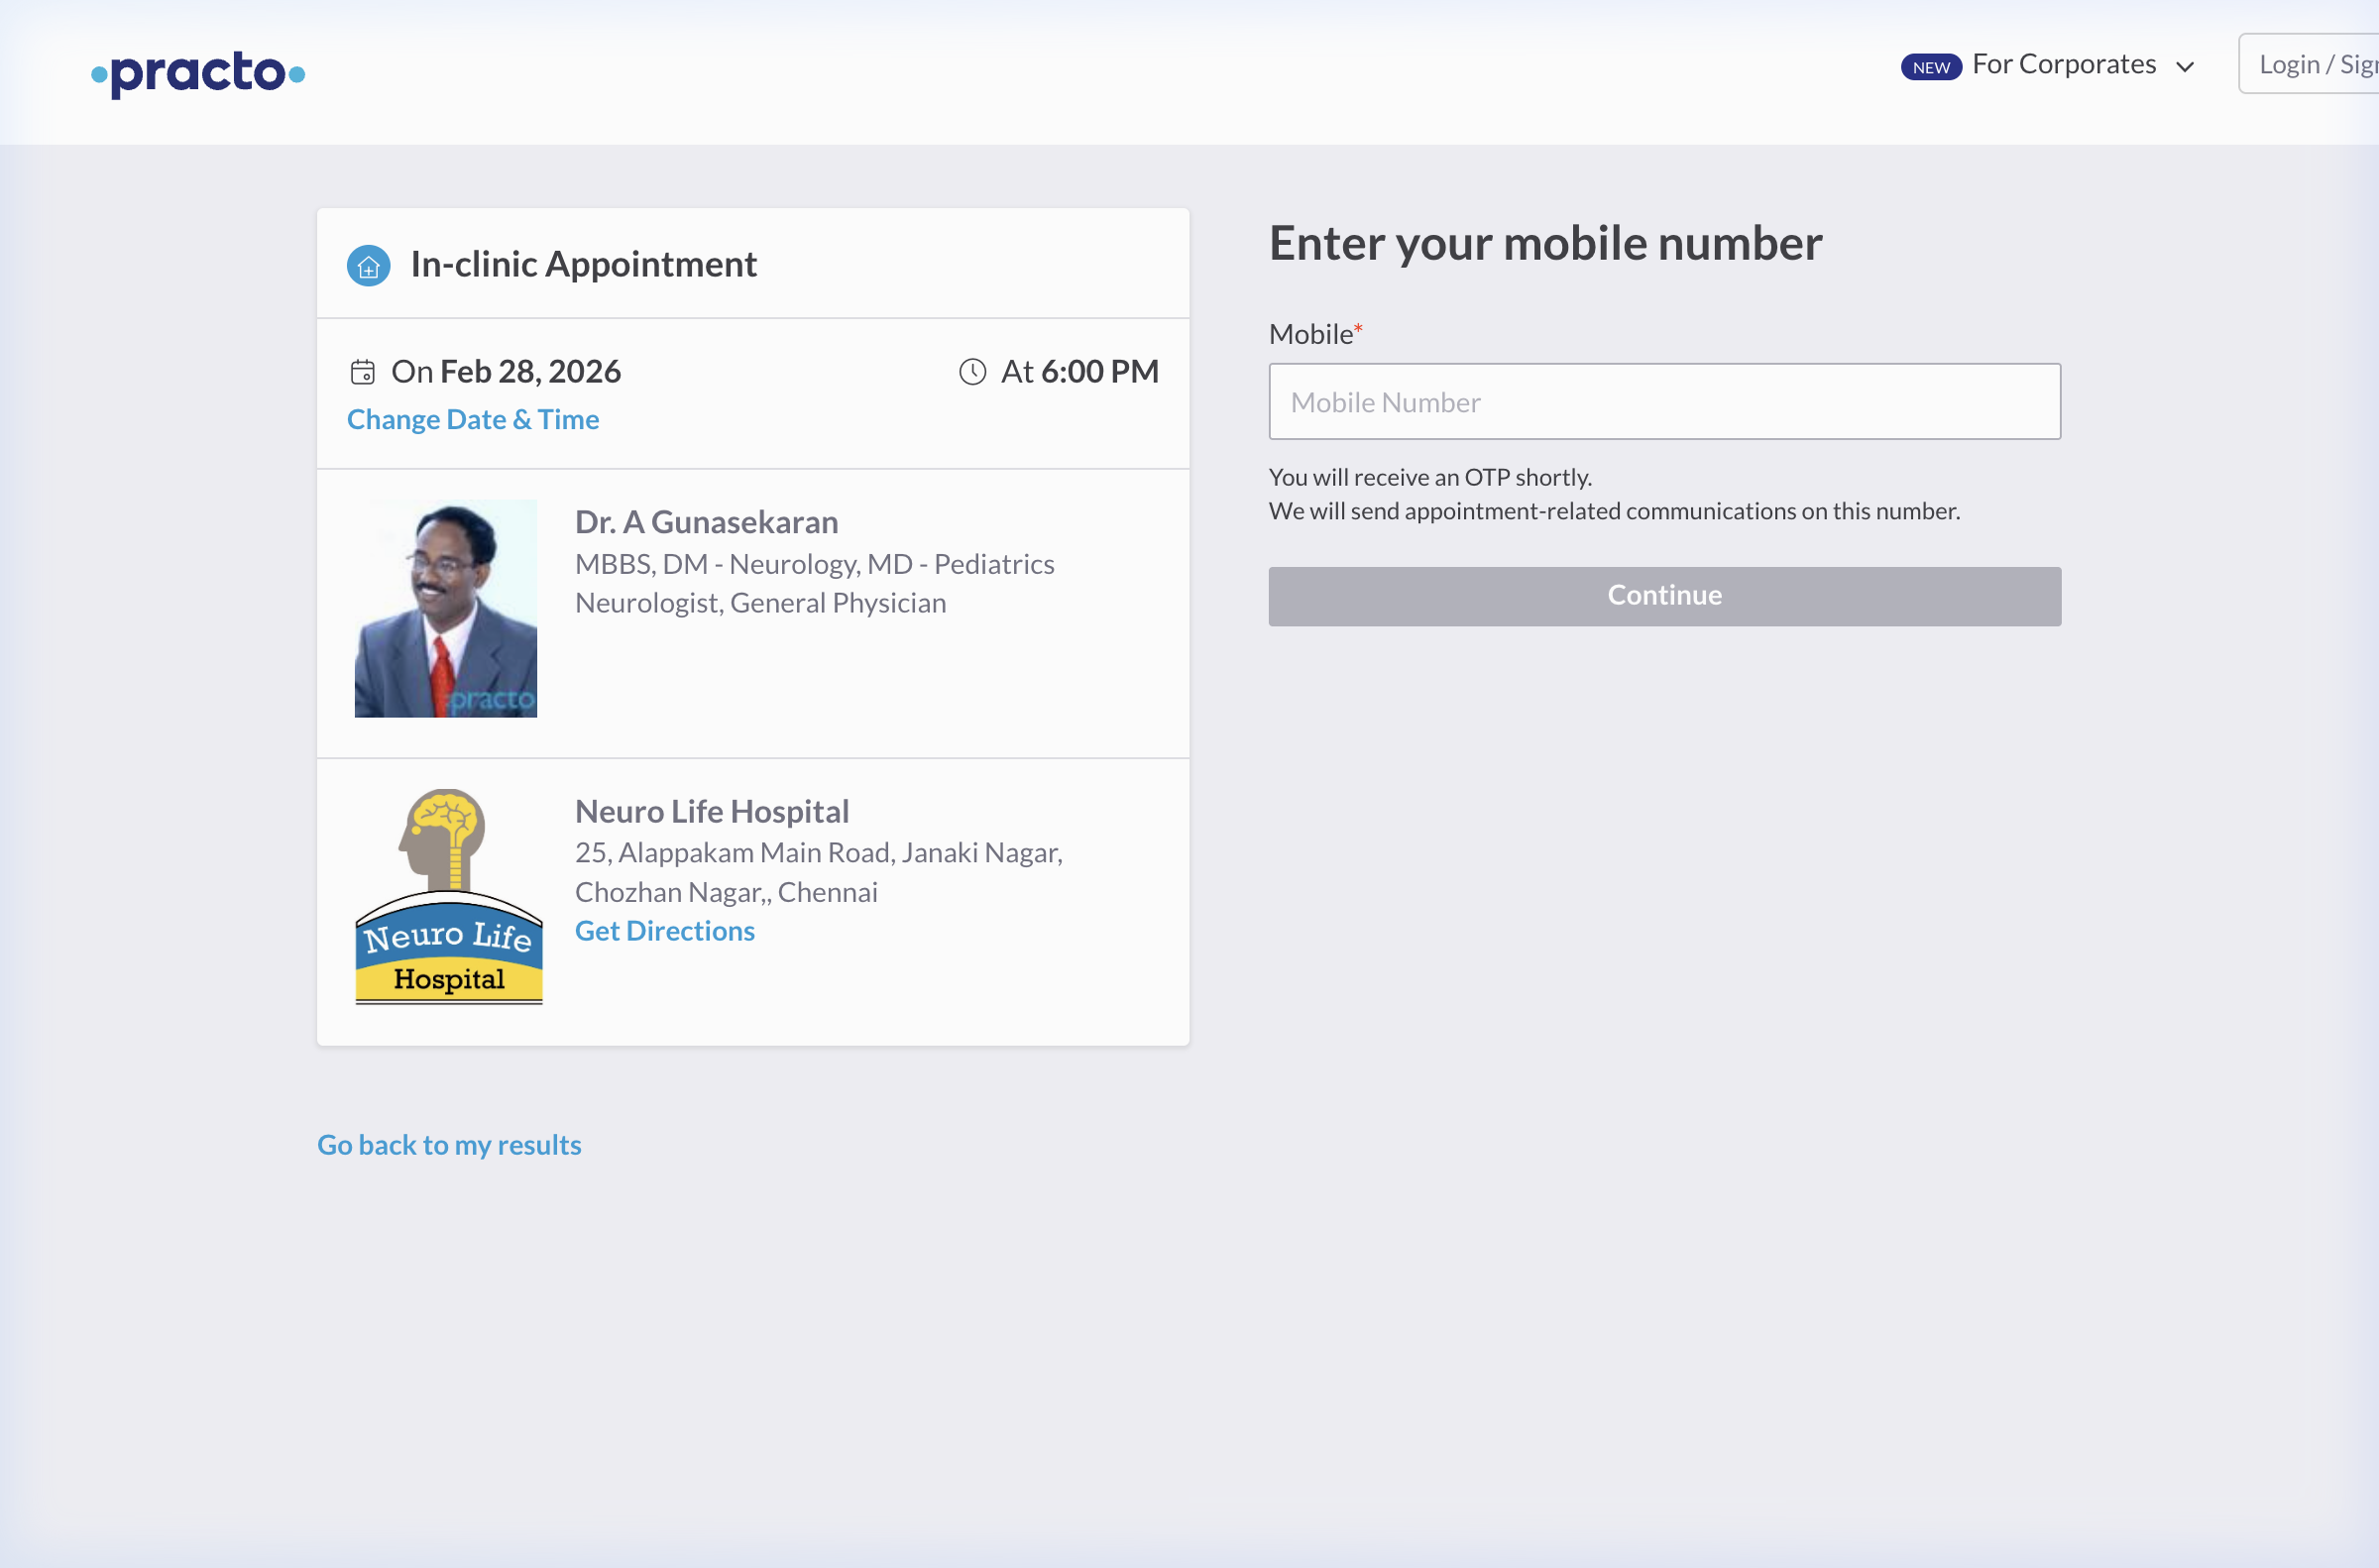
\includegraphics[width=\textwidth]{practo_booking.png}
        \caption{Details page --- no step count, greyed button}
    \end{subfigure}
    \caption{Practo's booking flow --- no progress indicator, weak feedback}
\end{figure}

\begin{hcibox}{Closure (Shneiderman \#4), Synthesizability, Shneiderman \#3 (Feedback), Shneiderman \#5 (Easy Reversal), Reset Must Die}
\textbf{Closure} (Shneiderman \#4) requires that sequences of actions have a clear beginning, middle, and end with informative feedback at completion. \textbf{Synthesizability} (Learnability sub-principle) requires users to be able to assess the effect of past operations and see where they are. \textbf{Shneiderman \#3} demands informative feedback for every action. \textbf{Shneiderman \#5} (Easy Reversal) means users should be able to go back. \textbf{Reset Must Die} --- forms should not have a ``Reset All'' button; instead, individual fields should be clearable.
\end{hcibox}

\begin{solutionbox}
Our booking flow has a \textbf{3-step progress bar} with clear labels: \textit{Select Slot $\rightarrow$ Confirm $\rightarrow$ Booked!}

Key features:
\begin{itemize}[leftmargin=*]
    \item \textbf{Progress indicator}: Step numbers (1/3, 2/3, 3/3) with connecting bar that fills as user progresses
    \item \textbf{Reversal of actions}: ``$\leftarrow$ Change Slot'' button on Step 2 allows going back to Step 1 (Shneiderman \#5)
    \item \textbf{No Reset button}: Individual field clear ($\times$) buttons instead of a destructive ``Reset All'' (Reset Must Die)
    \item \textbf{Success animation}: Green checkmark with confirmation summary on Step 3 (Closure)
    \item \textbf{Loading feedback}: Spinner with ``Booking...'' text during submission (Shneiderman \#3)
\end{itemize}
\end{solutionbox}

\textit{Screenshot: Navigate to any doctor profile $\rightarrow$ ``Book Appointment'' $\rightarrow$ follow the 3-step flow.}

% TODO: Replace with actual screenshots of booking steps 1, 2, 3
% \begin{figure}[H]
%     \centering
%     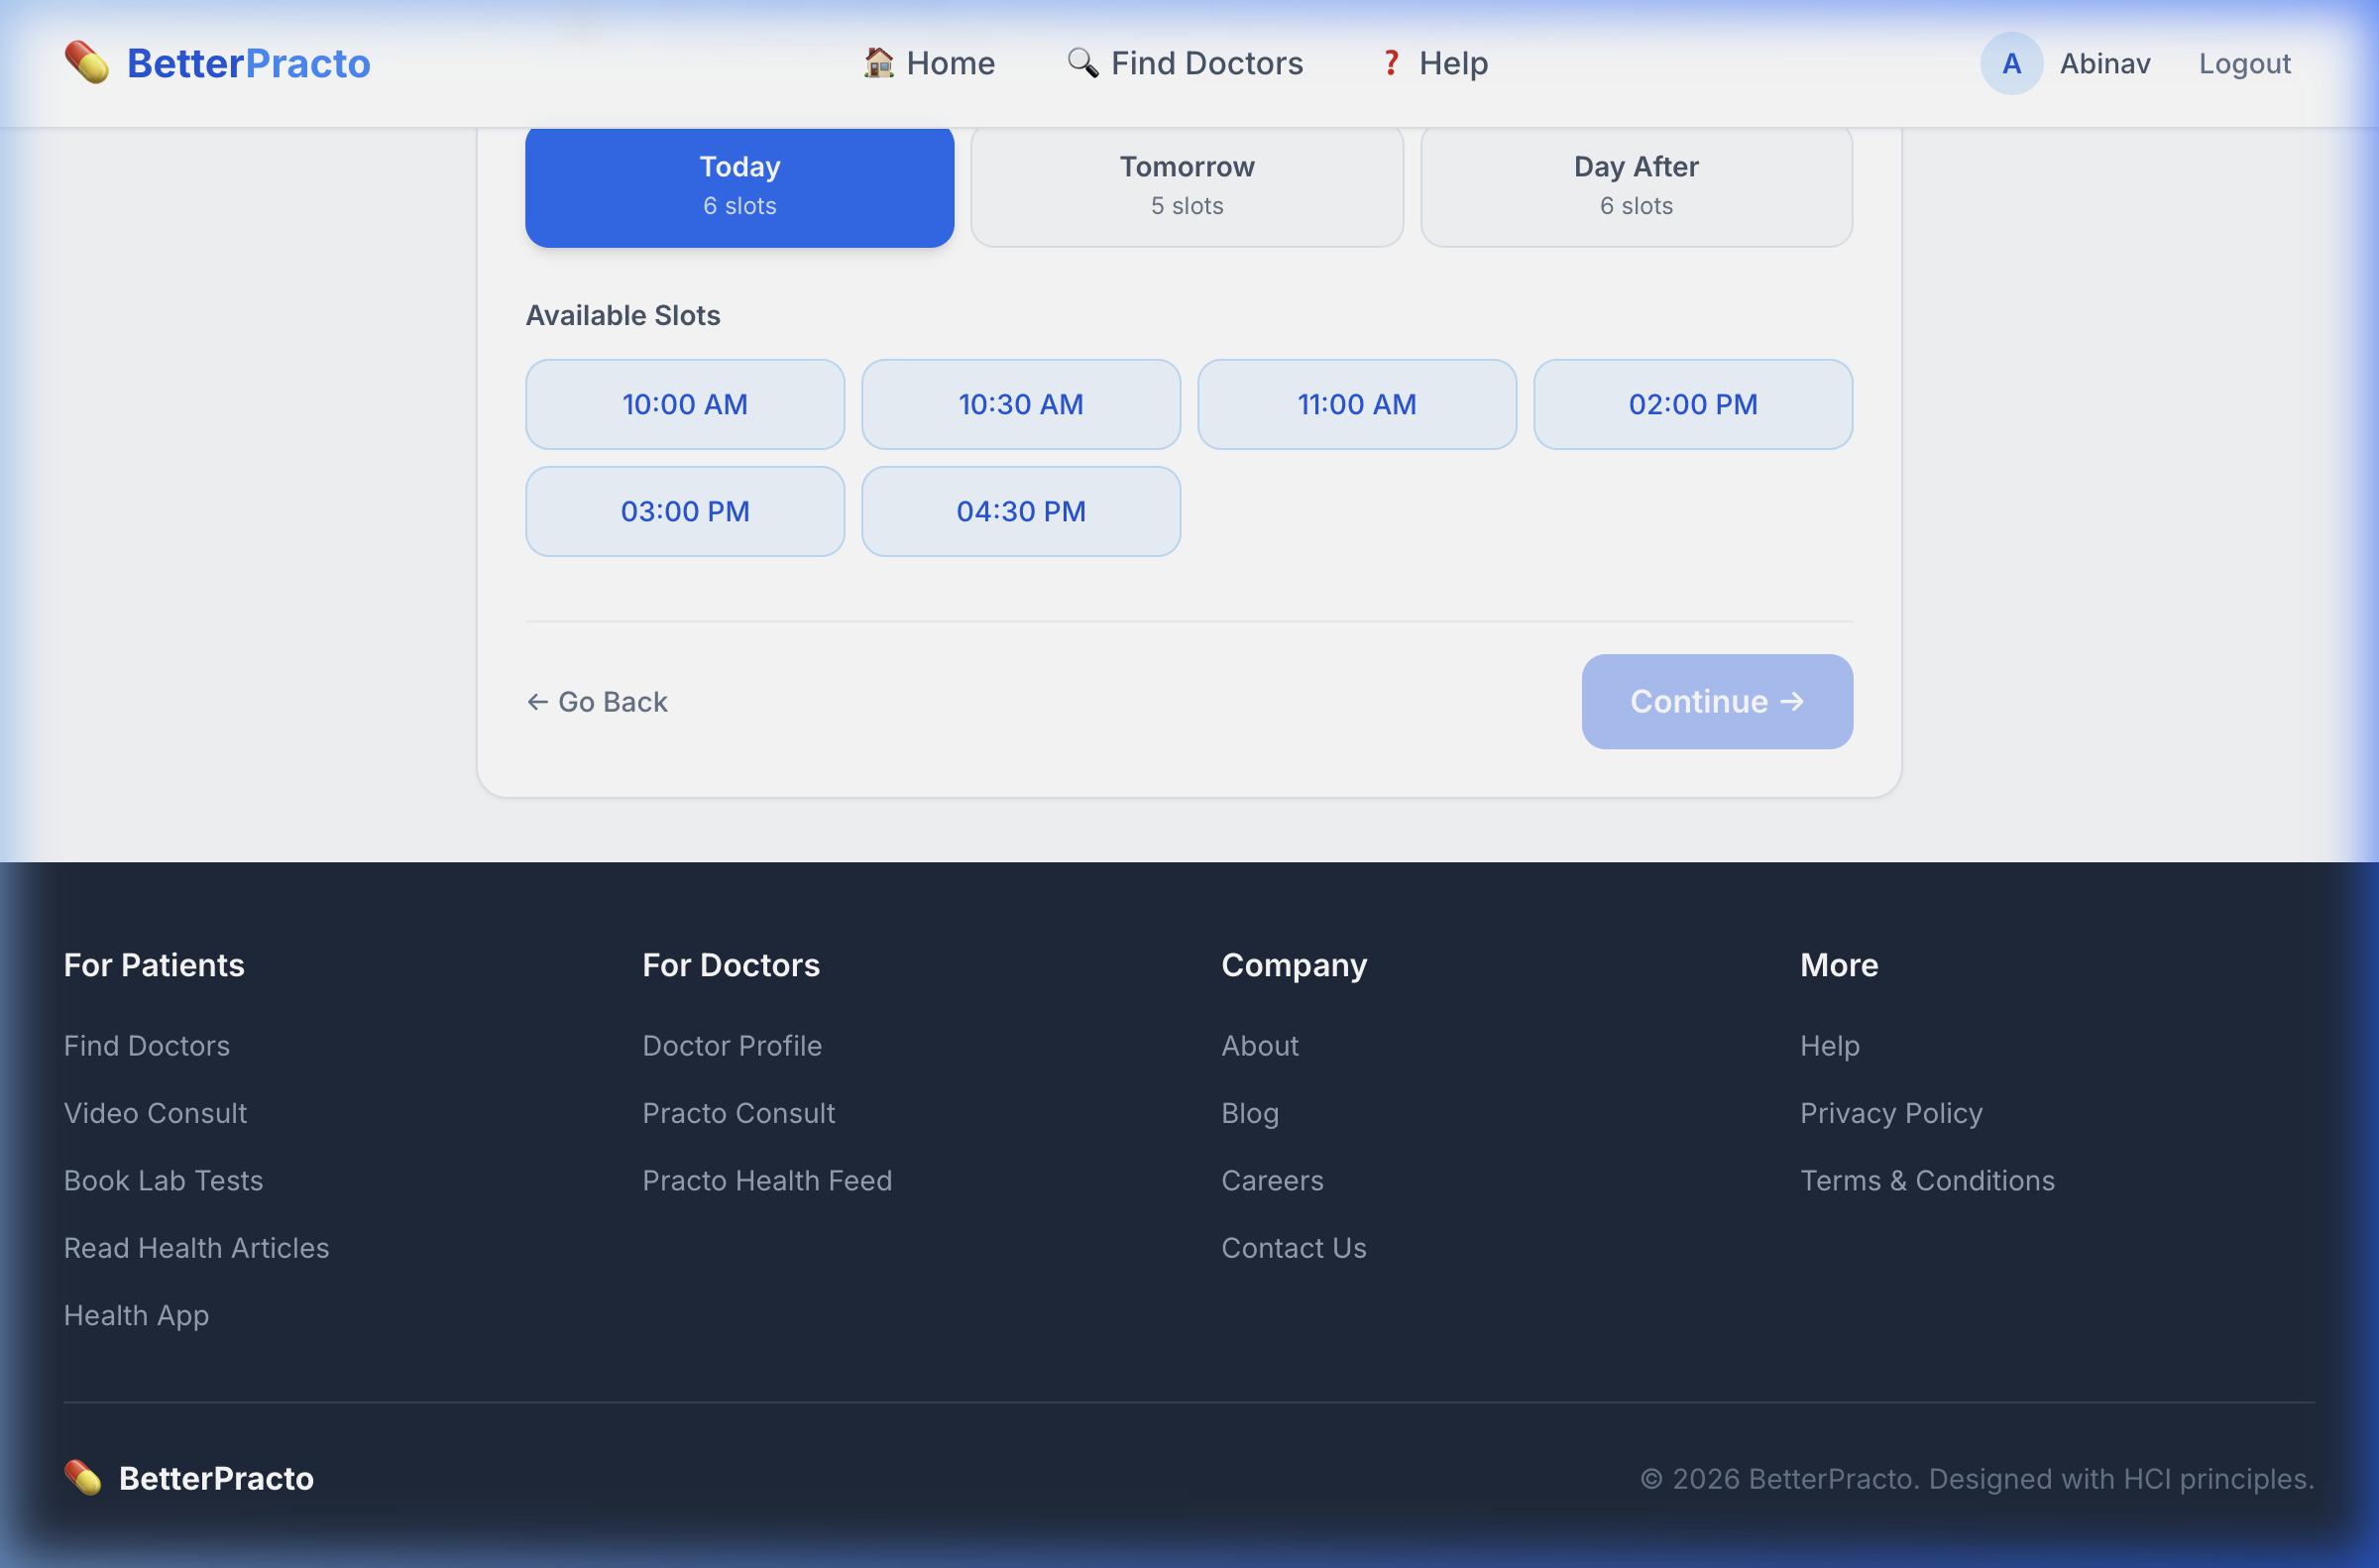
\includegraphics[width=\textwidth]{our_booking_step1.png}
%     \caption{Better Practo --- Step 1 with progress bar and slot selection}
% \end{figure}
% \begin{figure}[H]
%     \centering
%     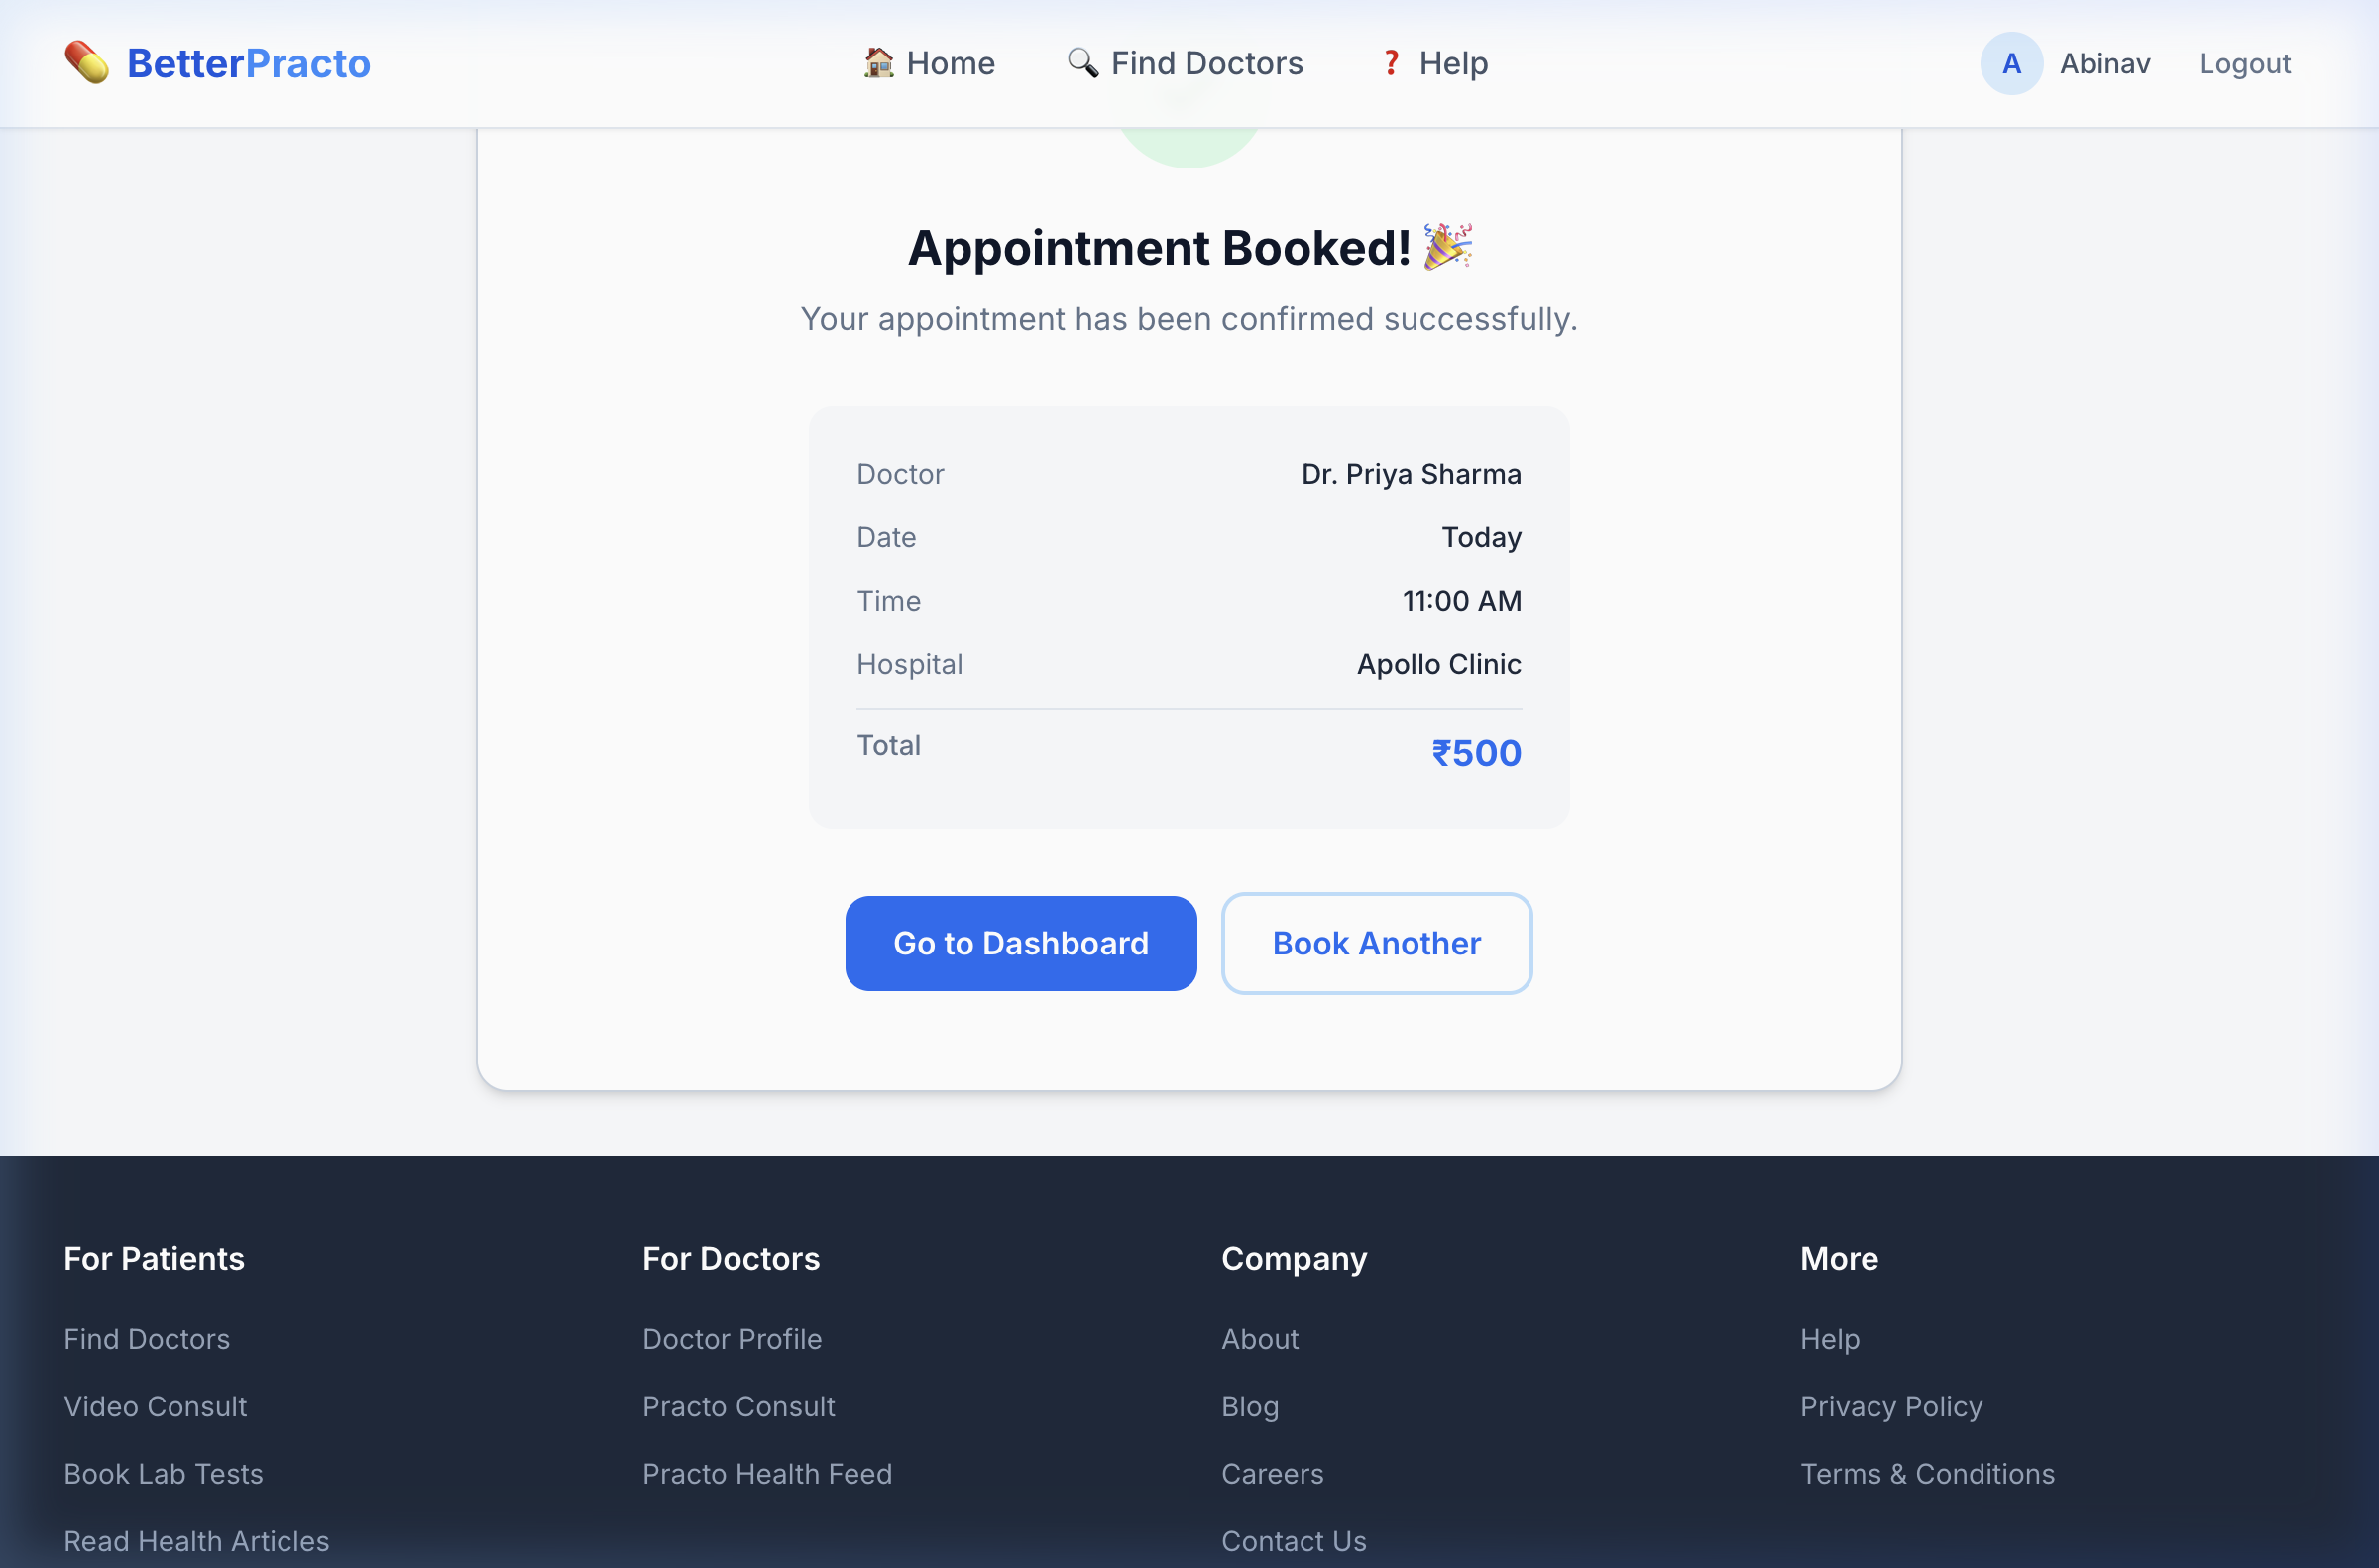
\includegraphics[width=\textwidth]{our_booking_step3.png}
%     \caption{Better Practo --- Step 3 success with confirmation animation (Closure)}
% \end{figure}

\newpage

% ----------------------------------------------------------------
\subsection{V8: Inconsistent Active Navigation State}

\begin{violationbox}
Practo's navigation bar shows an active state (blue underline) on \textit{some} pages (e.g., ``Find Doctors'' on the search page) but \textbf{not on others} (e.g., the homepage has no highlighted nav item). This inconsistency violates the principle that users should always know where they are.
\end{violationbox}

\begin{hcibox}{Nielsen \#1 (Visibility of System Status), Consistency (Shneiderman \#1)}
\textbf{Nielsen \#1} states the system should always keep users informed about what is going on. An active nav state tells users \textit{where they are} in the app. \textbf{Shneiderman \#1} (Consistency) means similar situations should use consistent visual cues --- if some pages highlight the active tab, all should.
\end{hcibox}

\begin{solutionbox}
Our navbar \textbf{consistently highlights the active page} on every route: blue background + bottom border for the current section. This works on Home, Find Doctors, and Help --- \textbf{no exceptions}.
\end{solutionbox}

\textit{Screenshot: Navigate between Home, Find Doctors, and Help --- observe the active state change consistently.}

% TODO: Replace with actual screenshot
% \begin{figure}[H]
%     \centering
%     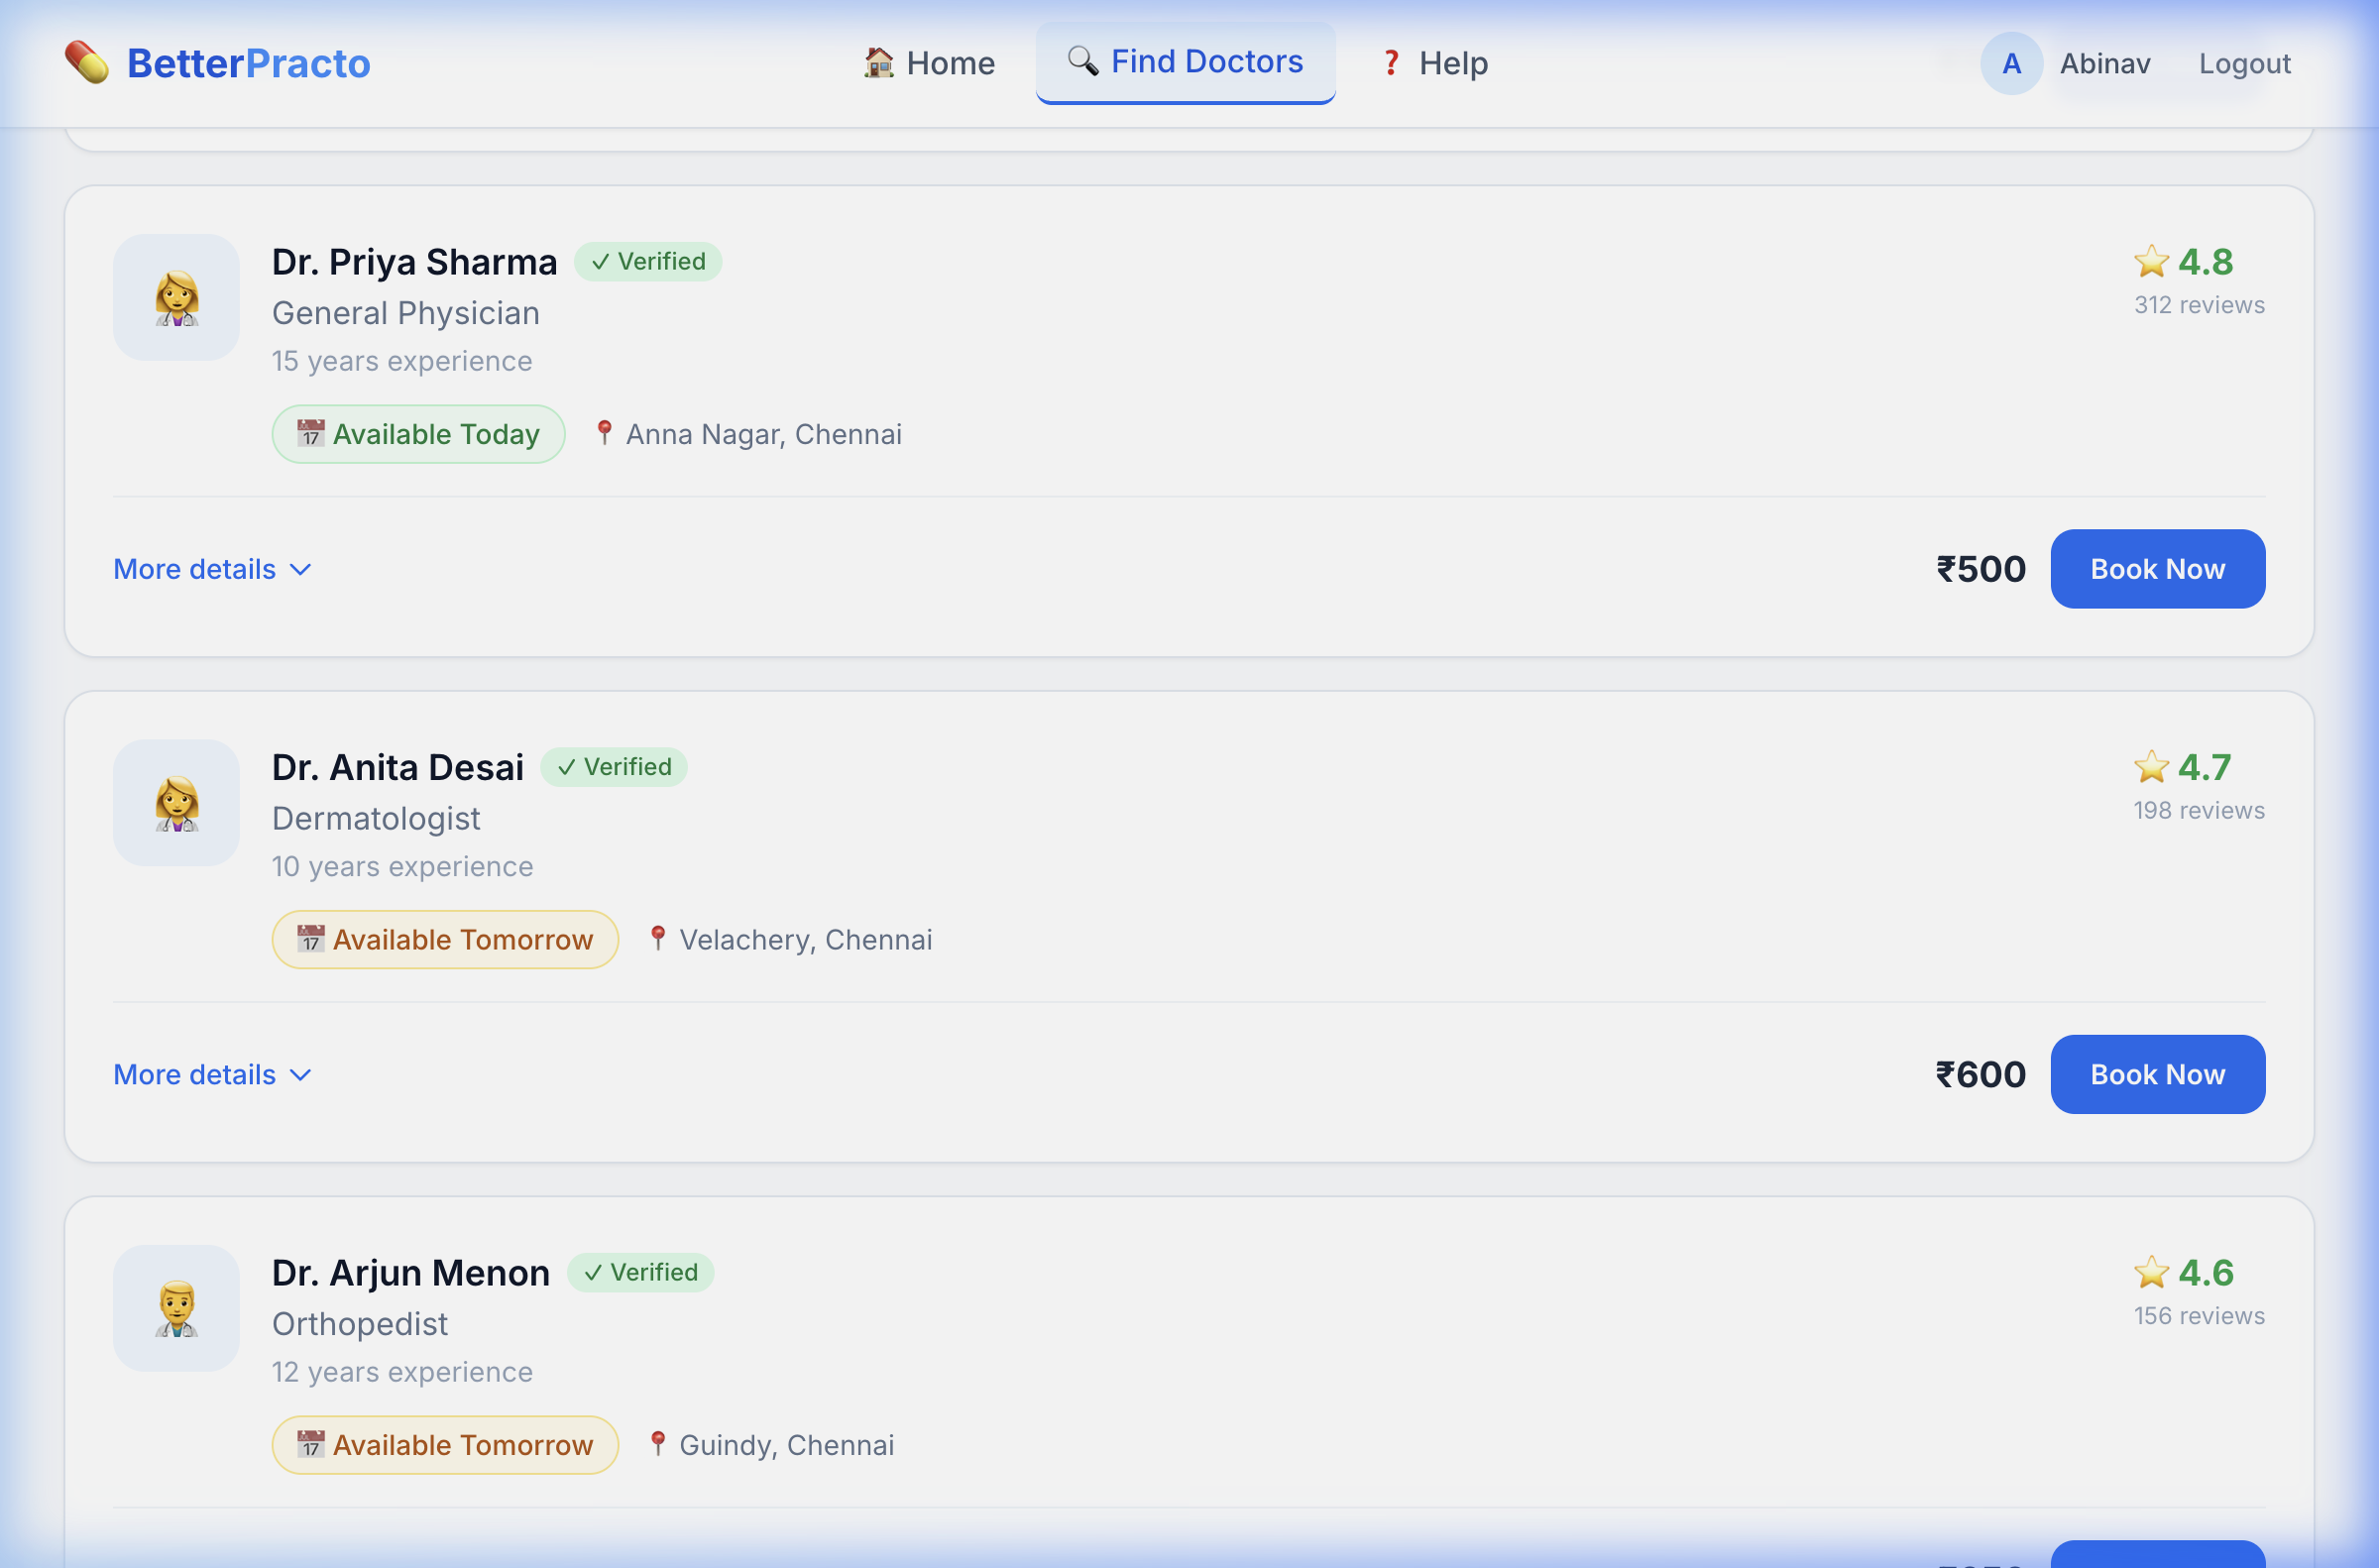
\includegraphics[width=0.8\textwidth]{our_navbar_active.png}
%     \caption{Better Practo --- Consistent active nav state on every page}
% \end{figure}

\newpage

% ----------------------------------------------------------------
\subsection{V9: Password Fully Masked Without Toggle}

\begin{violationbox}
Practo's login masks the password completely with no option to reveal it. Users cannot verify what they typed, leading to errors and frustration, especially on mobile where typos are common.
\end{violationbox}

\begin{hcibox}{Stop Password Masking (Lecture 5 Case Study), Feedback (Norman), Error Prevention (Nielsen \#5)}
The \textbf{Stop Password Masking} case study (Lecture 5) argues that password masking causes more harm (typos, frustration, repeated attempts) than good (shoulder surfing is rare). \textbf{Norman's Feedback Rule} says users need to see the effect of their actions. \textbf{Nielsen \#5} (Error Prevention) --- letting users see their password prevents typos.
\end{hcibox}

\begin{solutionbox}
Our login includes a \textbf{show/hide password toggle} (eye icon). By default, the password is masked. Clicking the eye reveals the text so users can verify before submitting. This balances security with usability.
\end{solutionbox}

\begin{figure}[H]
    \centering
    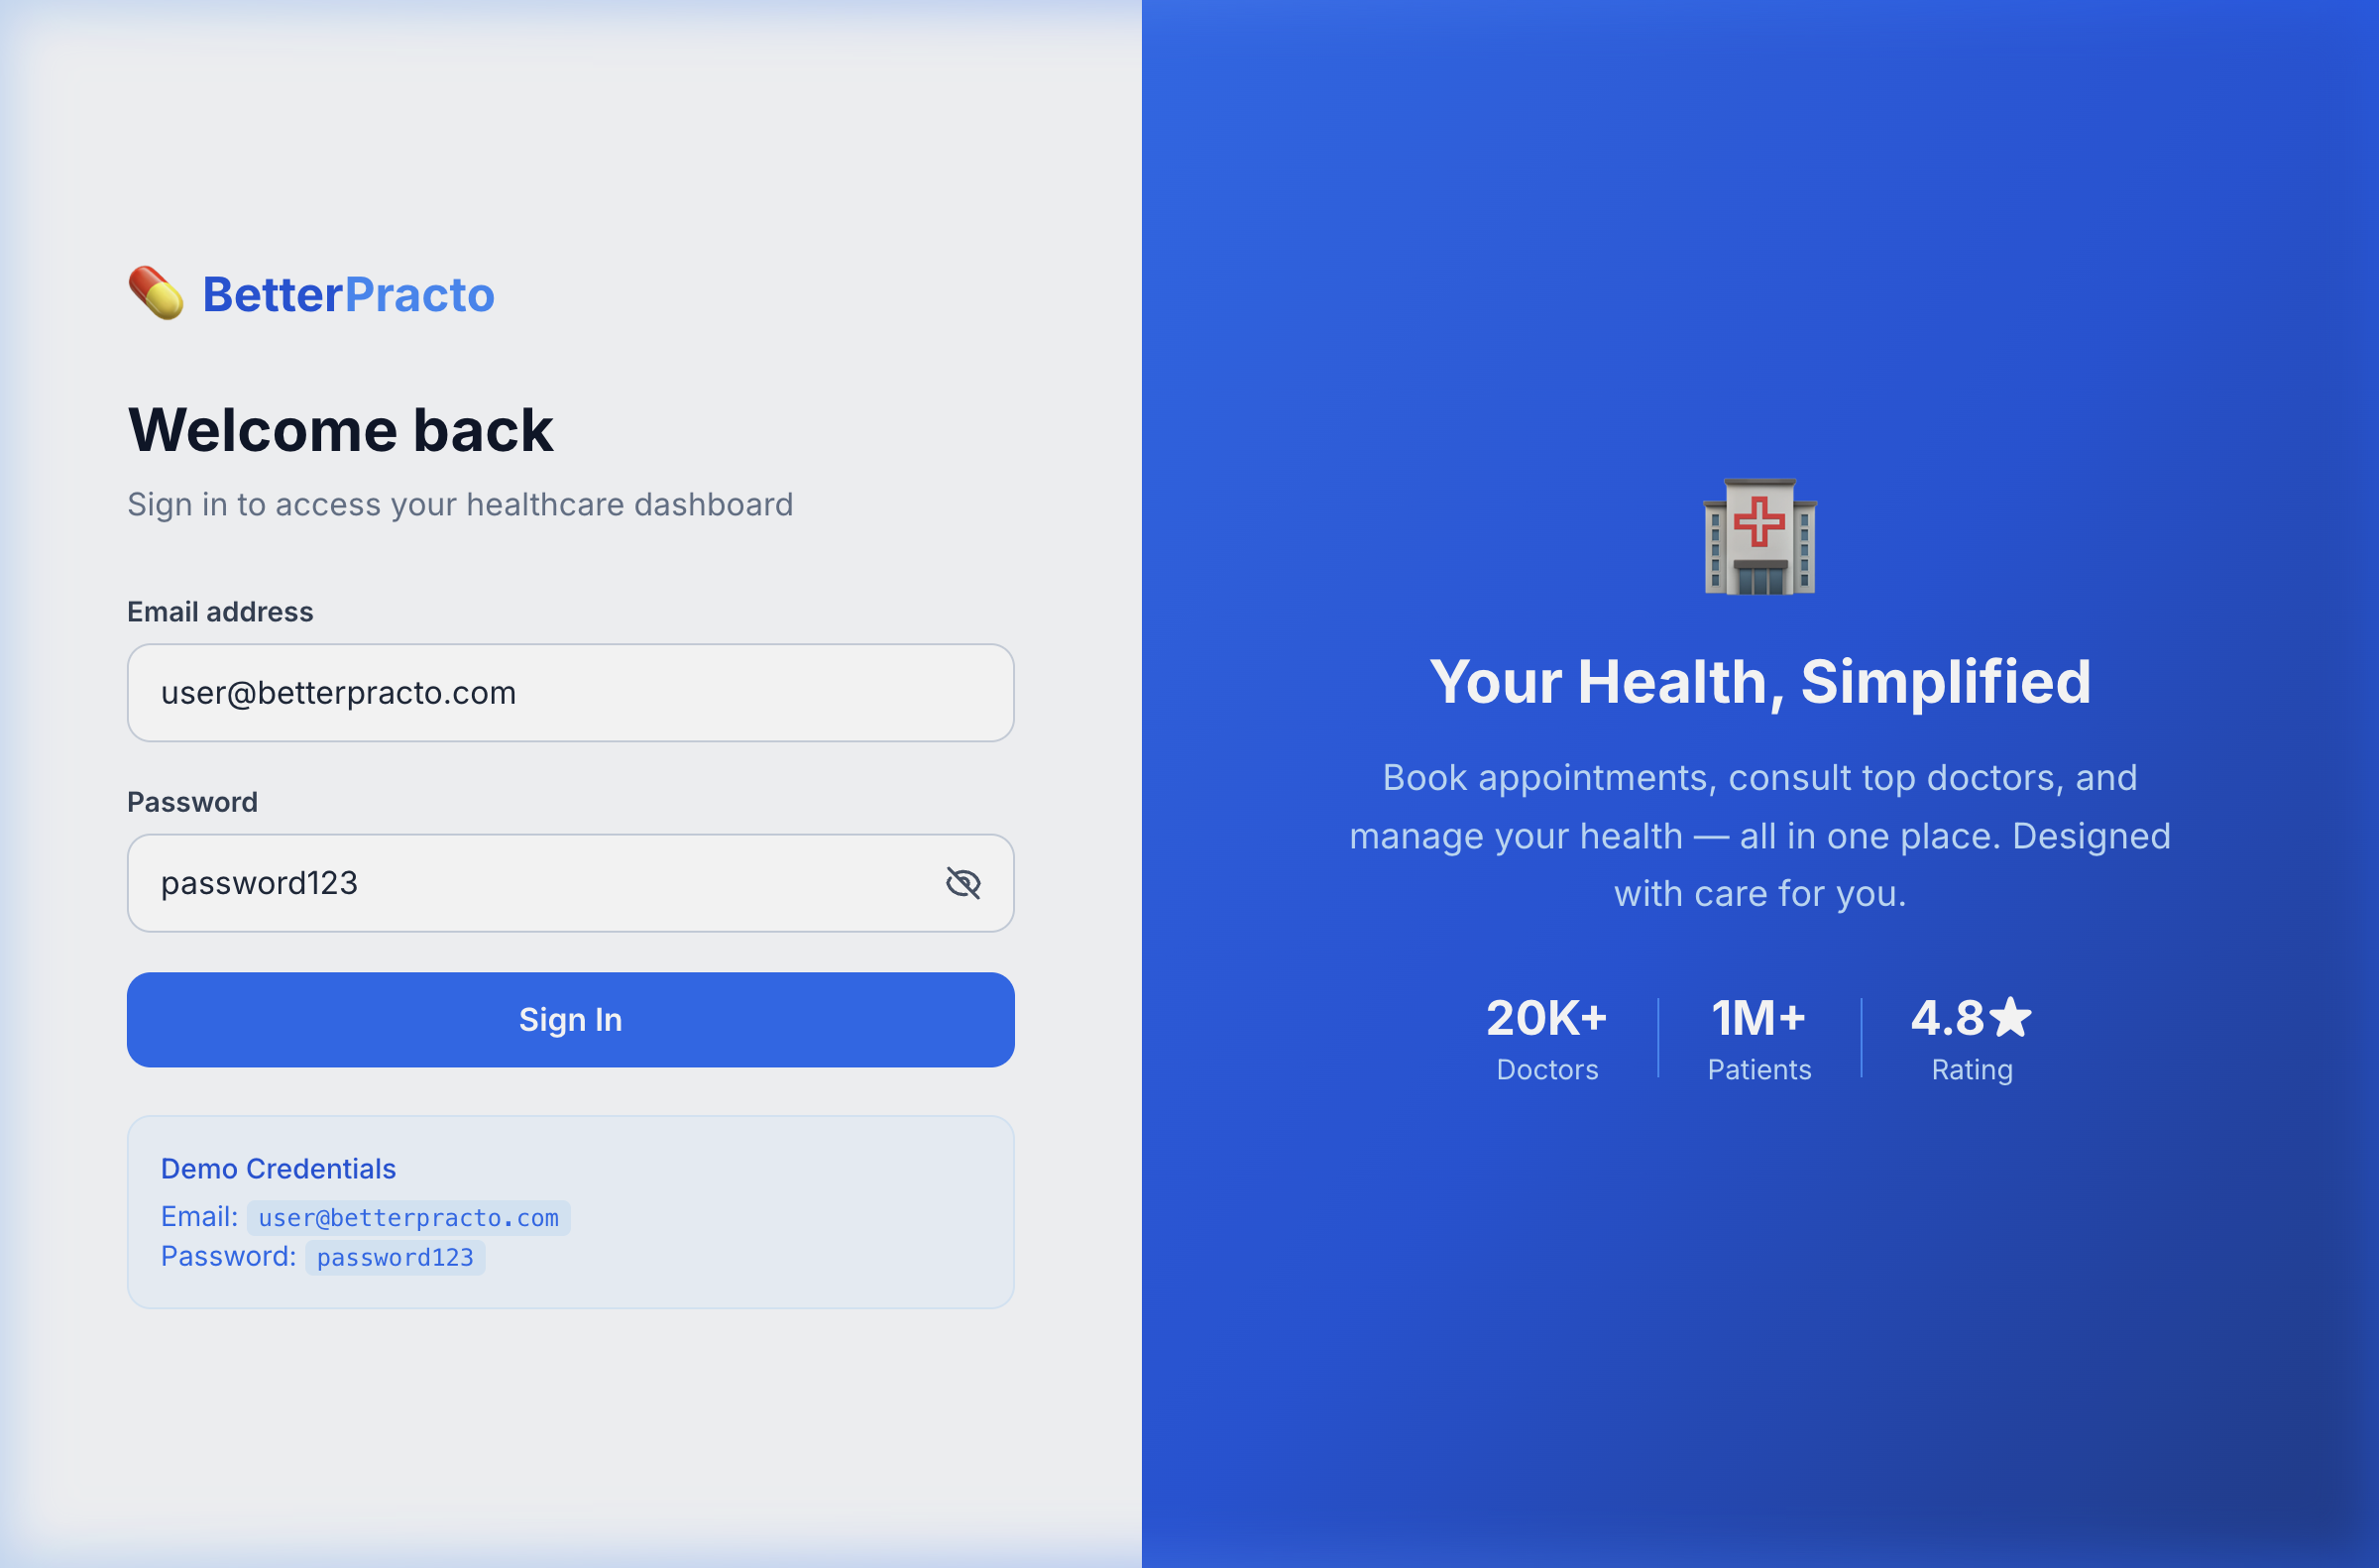
\includegraphics[width=0.9\textwidth]{our_login.png}
    \caption{Better Practo --- Show/hide password toggle (eye icon visible next to ``password123'')}
\end{figure}

\newpage

% ----------------------------------------------------------------
\subsection{V12: Default Sort is Unclear / Alphabetical}

\begin{violationbox}
Practo's search results default to ``Relevance'' but the sorting criteria is opaque and inconsistent. The \textbf{Alphabetical Sorting Must Die} case study argues that alphabetical ordering is almost never the best default for user-facing lists.
\end{violationbox}

\begin{hcibox}{Alphabetical Sorting Must Die (Lecture 6), Hick's Law}
\textbf{Alphabetical Sorting Must Die} (Lecture 6) argues that alphabetical order reflects the system's convenience, not the user's mental model. Users think in terms of \textit{best rated}, \textit{most experienced}, or \textit{cheapest} --- not alphabetical order. \textbf{Hick's Law} --- with clear sort options, decision time is reduced.
\end{hcibox}

\begin{solutionbox}
Our search results offer \textbf{explicit sort pills}: Relevance (default), Rating, Experience, Fee: Low to High. The active sort is visually highlighted with a filled blue button. No alphabetical option. Default is \textbf{Relevance} (rating $\times$ reviews).
\end{solutionbox}

\textit{See Figure 9 (search results screenshots) --- sort pills visible at top.}

\newpage

% ----------------------------------------------------------------
\subsection{V13: Forced City Selection Modal}

\begin{violationbox}
Practo's Lab Tests page forces a \textbf{city selection modal} before showing any content. The user cannot even browse available tests without first selecting a city. This wastes user time and adds an unnecessary step.
\end{violationbox}

\begin{figure}[H]
    \centering
    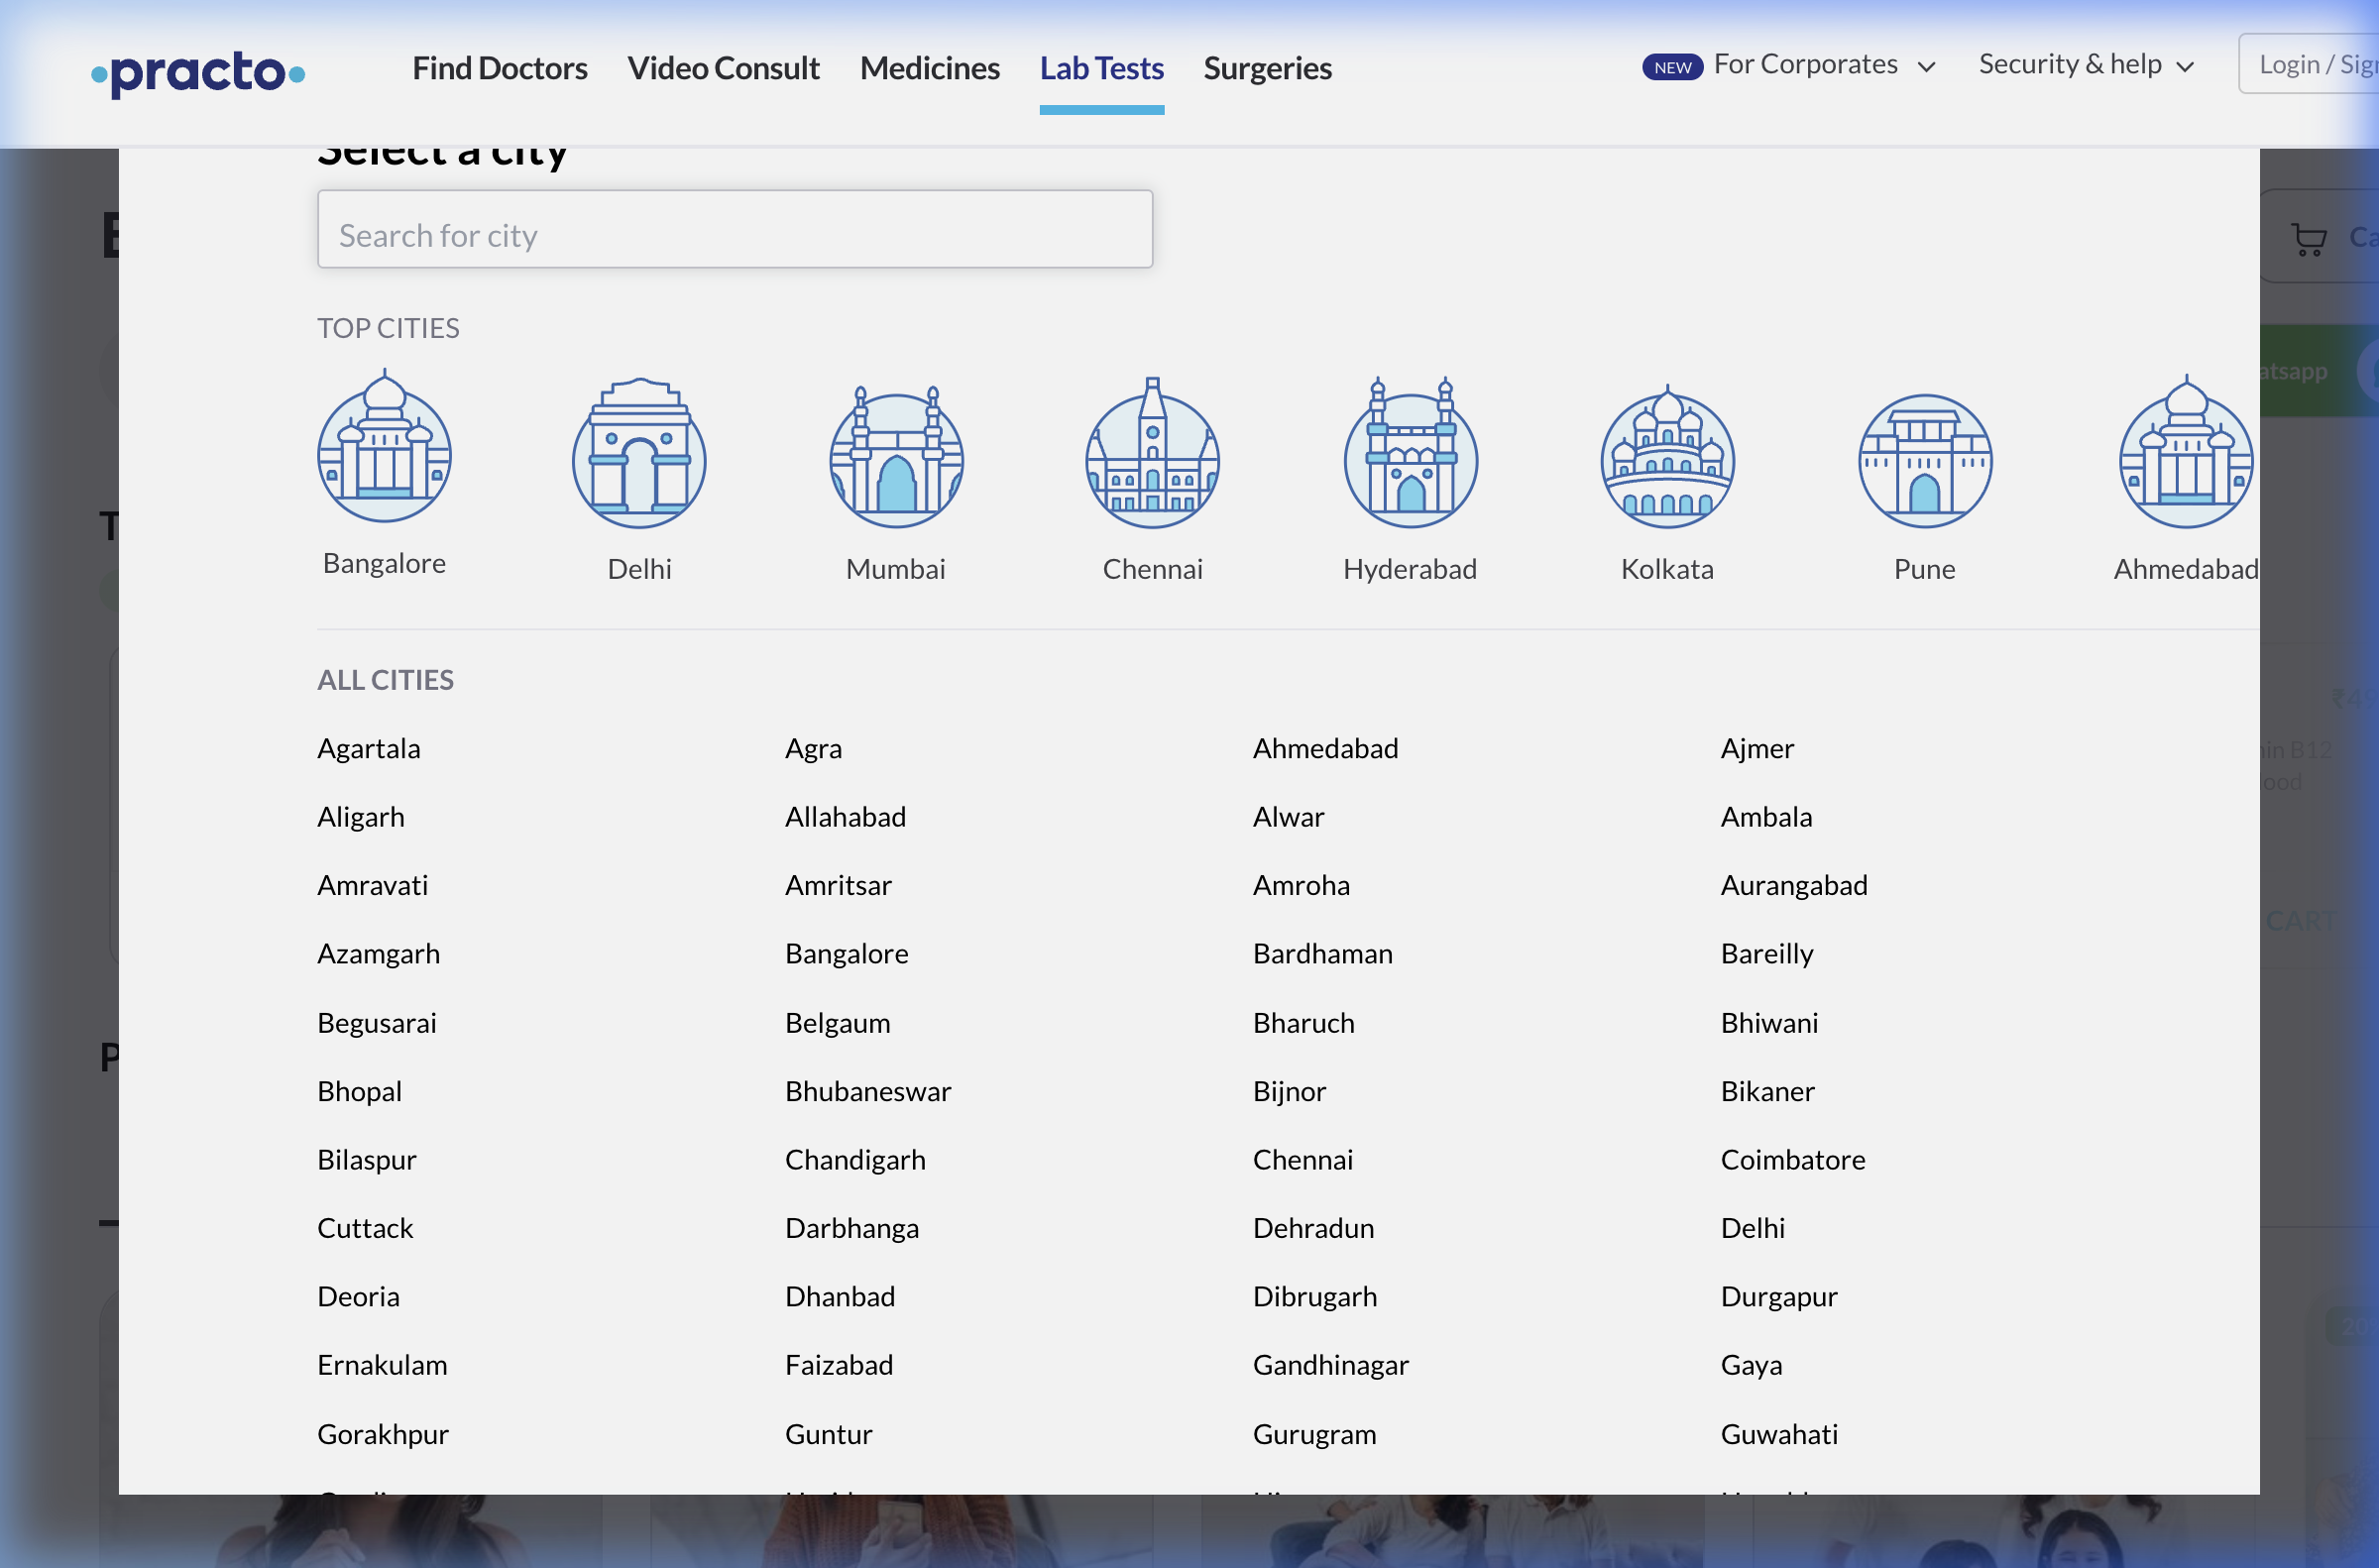
\includegraphics[width=0.6\textwidth]{practo_city_selection.png}
    \caption{Practo forces city selection before showing any content}
\end{figure}

\begin{hcibox}{Asimov's 2nd Law (Don't Waste Time), Zipf's Law (Least Effort)}
\textbf{Asimov's 2nd Law} adapted for HCI says the system should not waste the user's time --- if location can be detected automatically, it should be. \textbf{Zipf's Law} (Principle of Least Effort) says users will follow the path requiring minimal effort.
\end{hcibox}

\begin{solutionbox}
Our app \textbf{auto-detects the user's city} (shown as ``$\mathcircled{}$ Chennai'' chip in the search bar) and allows changing it with a single tap. No blocking modals, no forced selections. Content loads immediately.
\end{solutionbox}

\newpage

% ----------------------------------------------------------------
\subsection{V6: No Contextual Help System}

\begin{violationbox}
Practo's Help page is on a \textbf{separate subdomain} (\texttt{help.practo.com}), breaking the user's context. The FAQ content is dense and not categorized by user task, making it hard to find answers quickly.
\end{violationbox}

\begin{figure}[H]
    \centering
    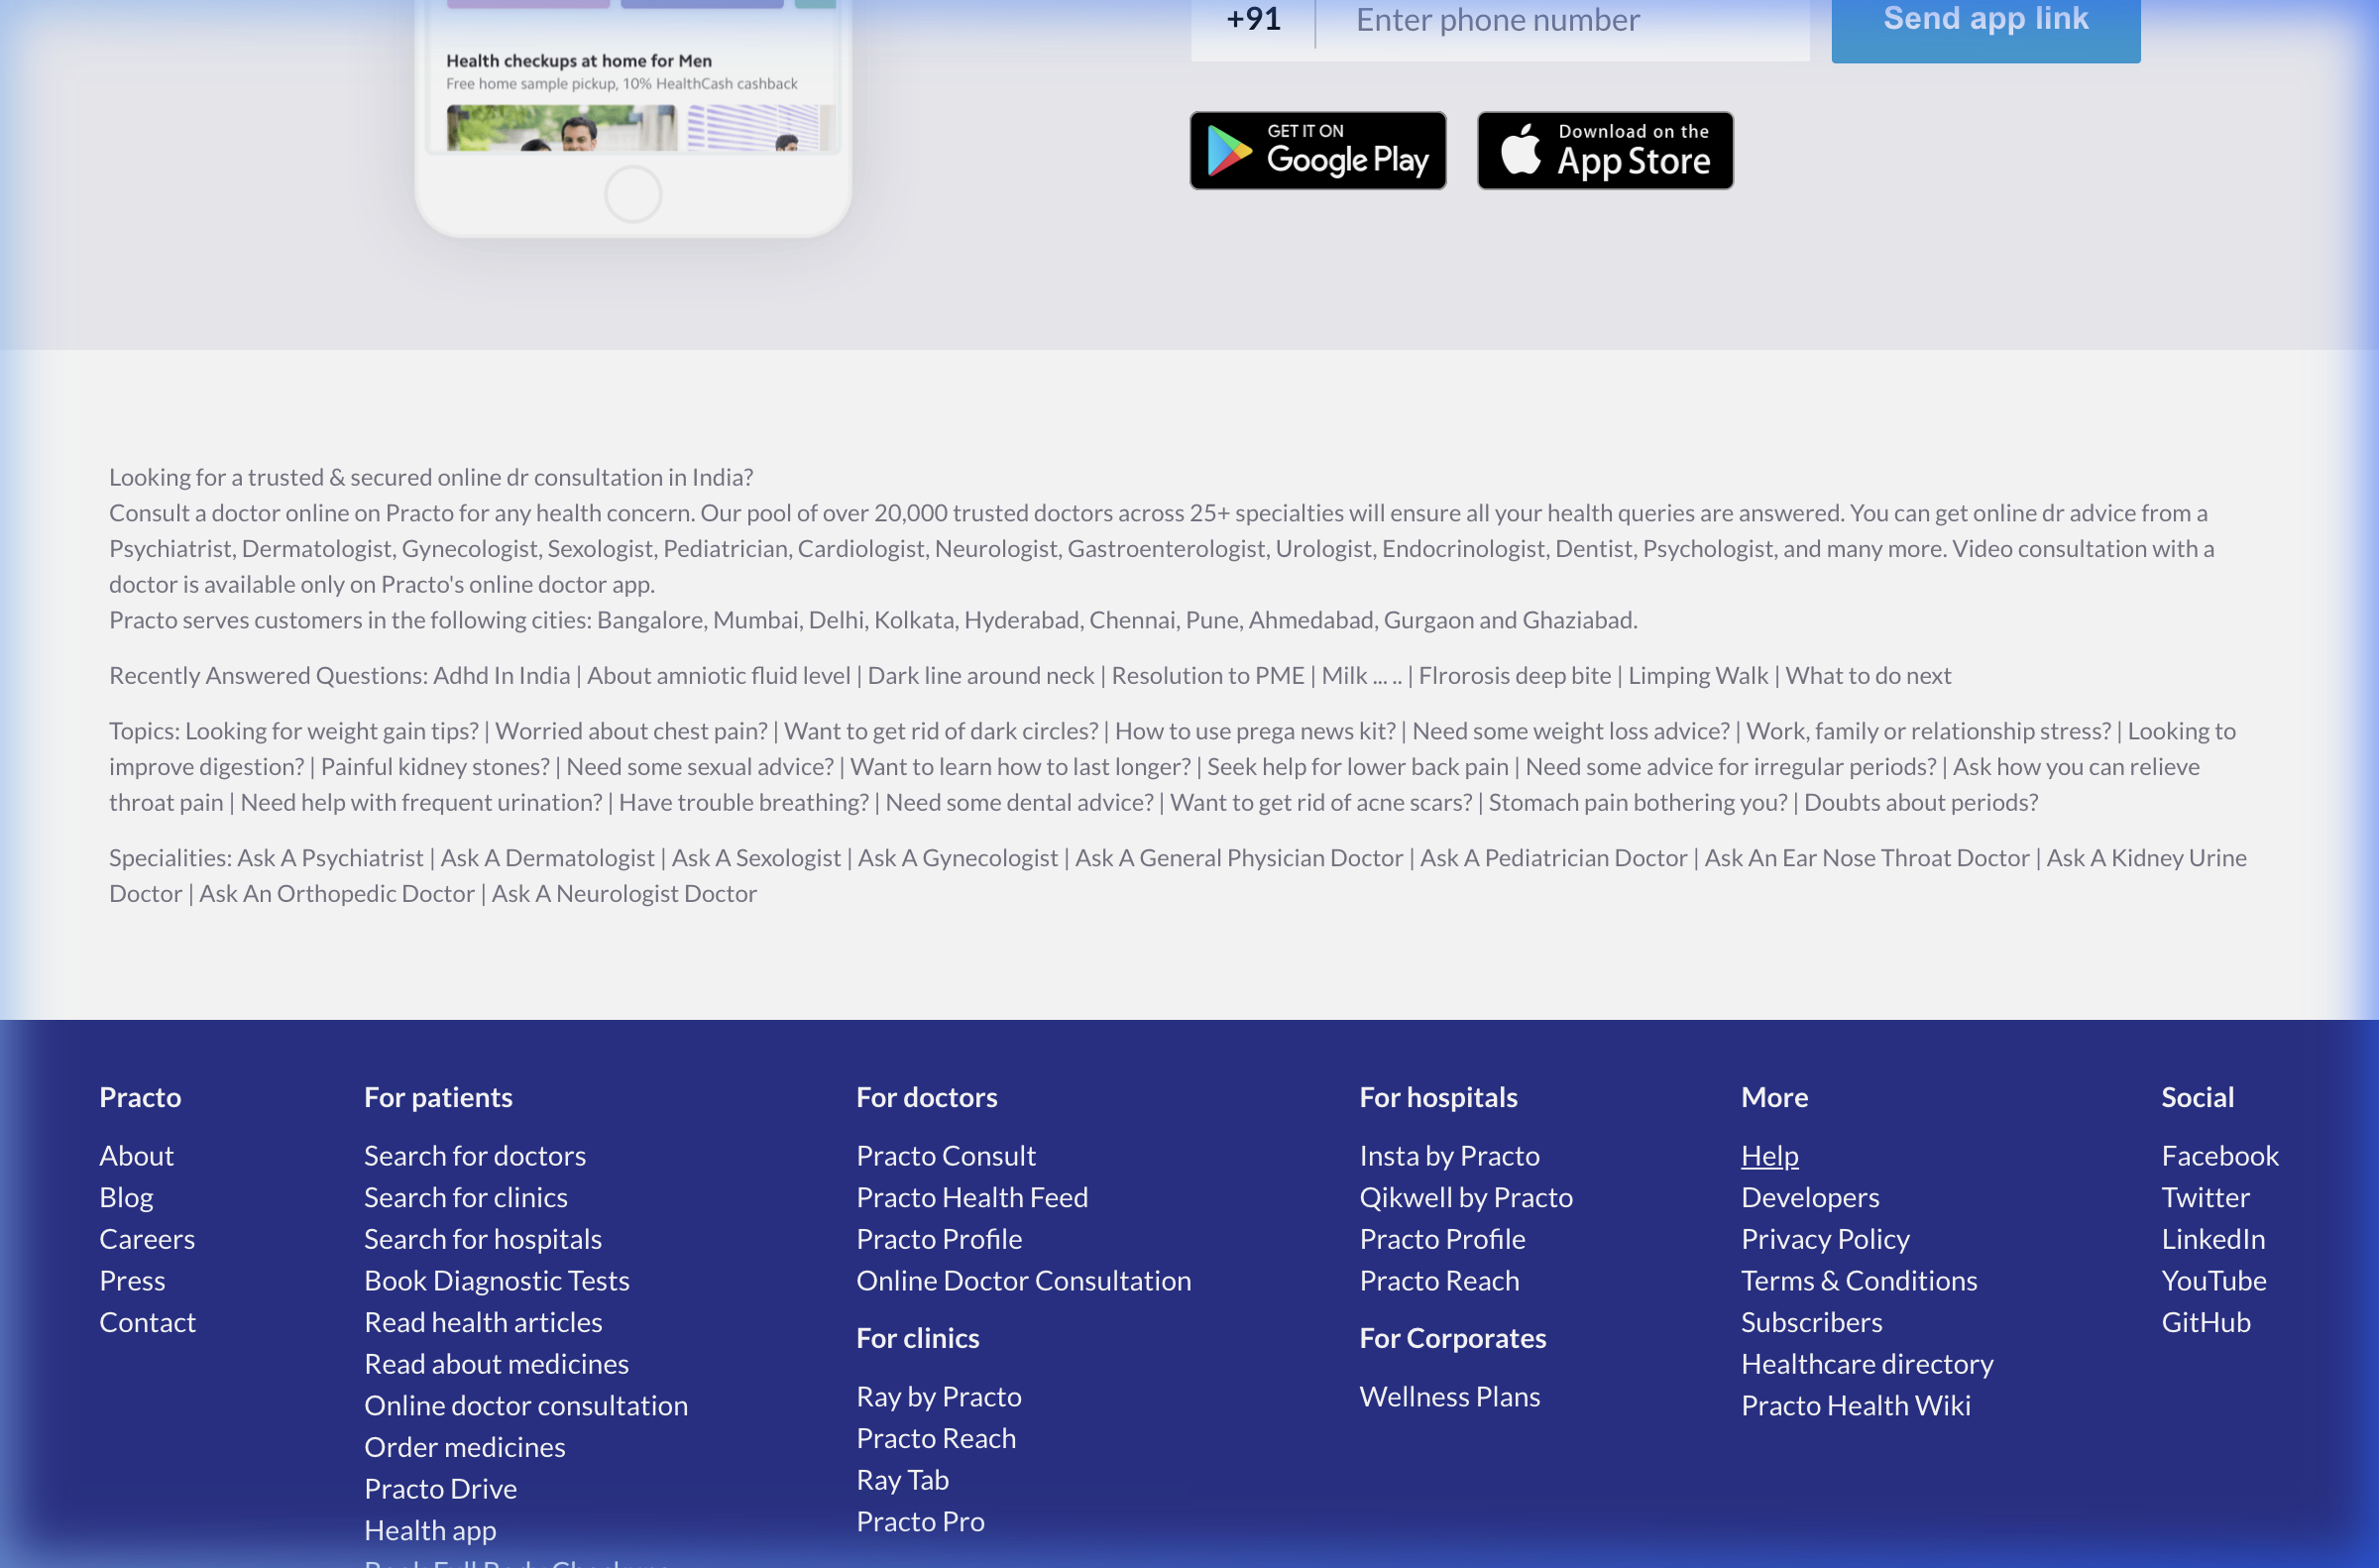
\includegraphics[width=0.8\textwidth]{practo_help.png}
    \caption{Practo's help page --- separate subdomain, dense FAQ listing}
\end{figure}

\begin{hcibox}{Nielsen \#10 (Help \& Documentation), Shneiderman \#8 (Reduce STM Load), Headline Usability}
\textbf{Nielsen \#10} says help should be easy to search, focused on the user's task, and not too large. \textbf{Shneiderman \#8} says the interface should reduce short-term memory demands. \textbf{Headline Usability} (Lecture 6) says headlines should be front-loaded and concise.
\end{hcibox}

\begin{solutionbox}
Our Help page is \textbf{built into the app} (same domain, accessible from navbar). FAQs are \textbf{categorized by user task} (Booking, Consultations, Payments, Privacy) with a \textbf{searchable input}. Questions use front-loaded, concise headlines and answers are in an accordion.
\end{solutionbox}

\textit{Screenshot: Click ``Help'' in the navbar to see the in-app searchable FAQ.}

% TODO: Replace with actual screenshot
% \begin{figure}[H]
%     \centering
%     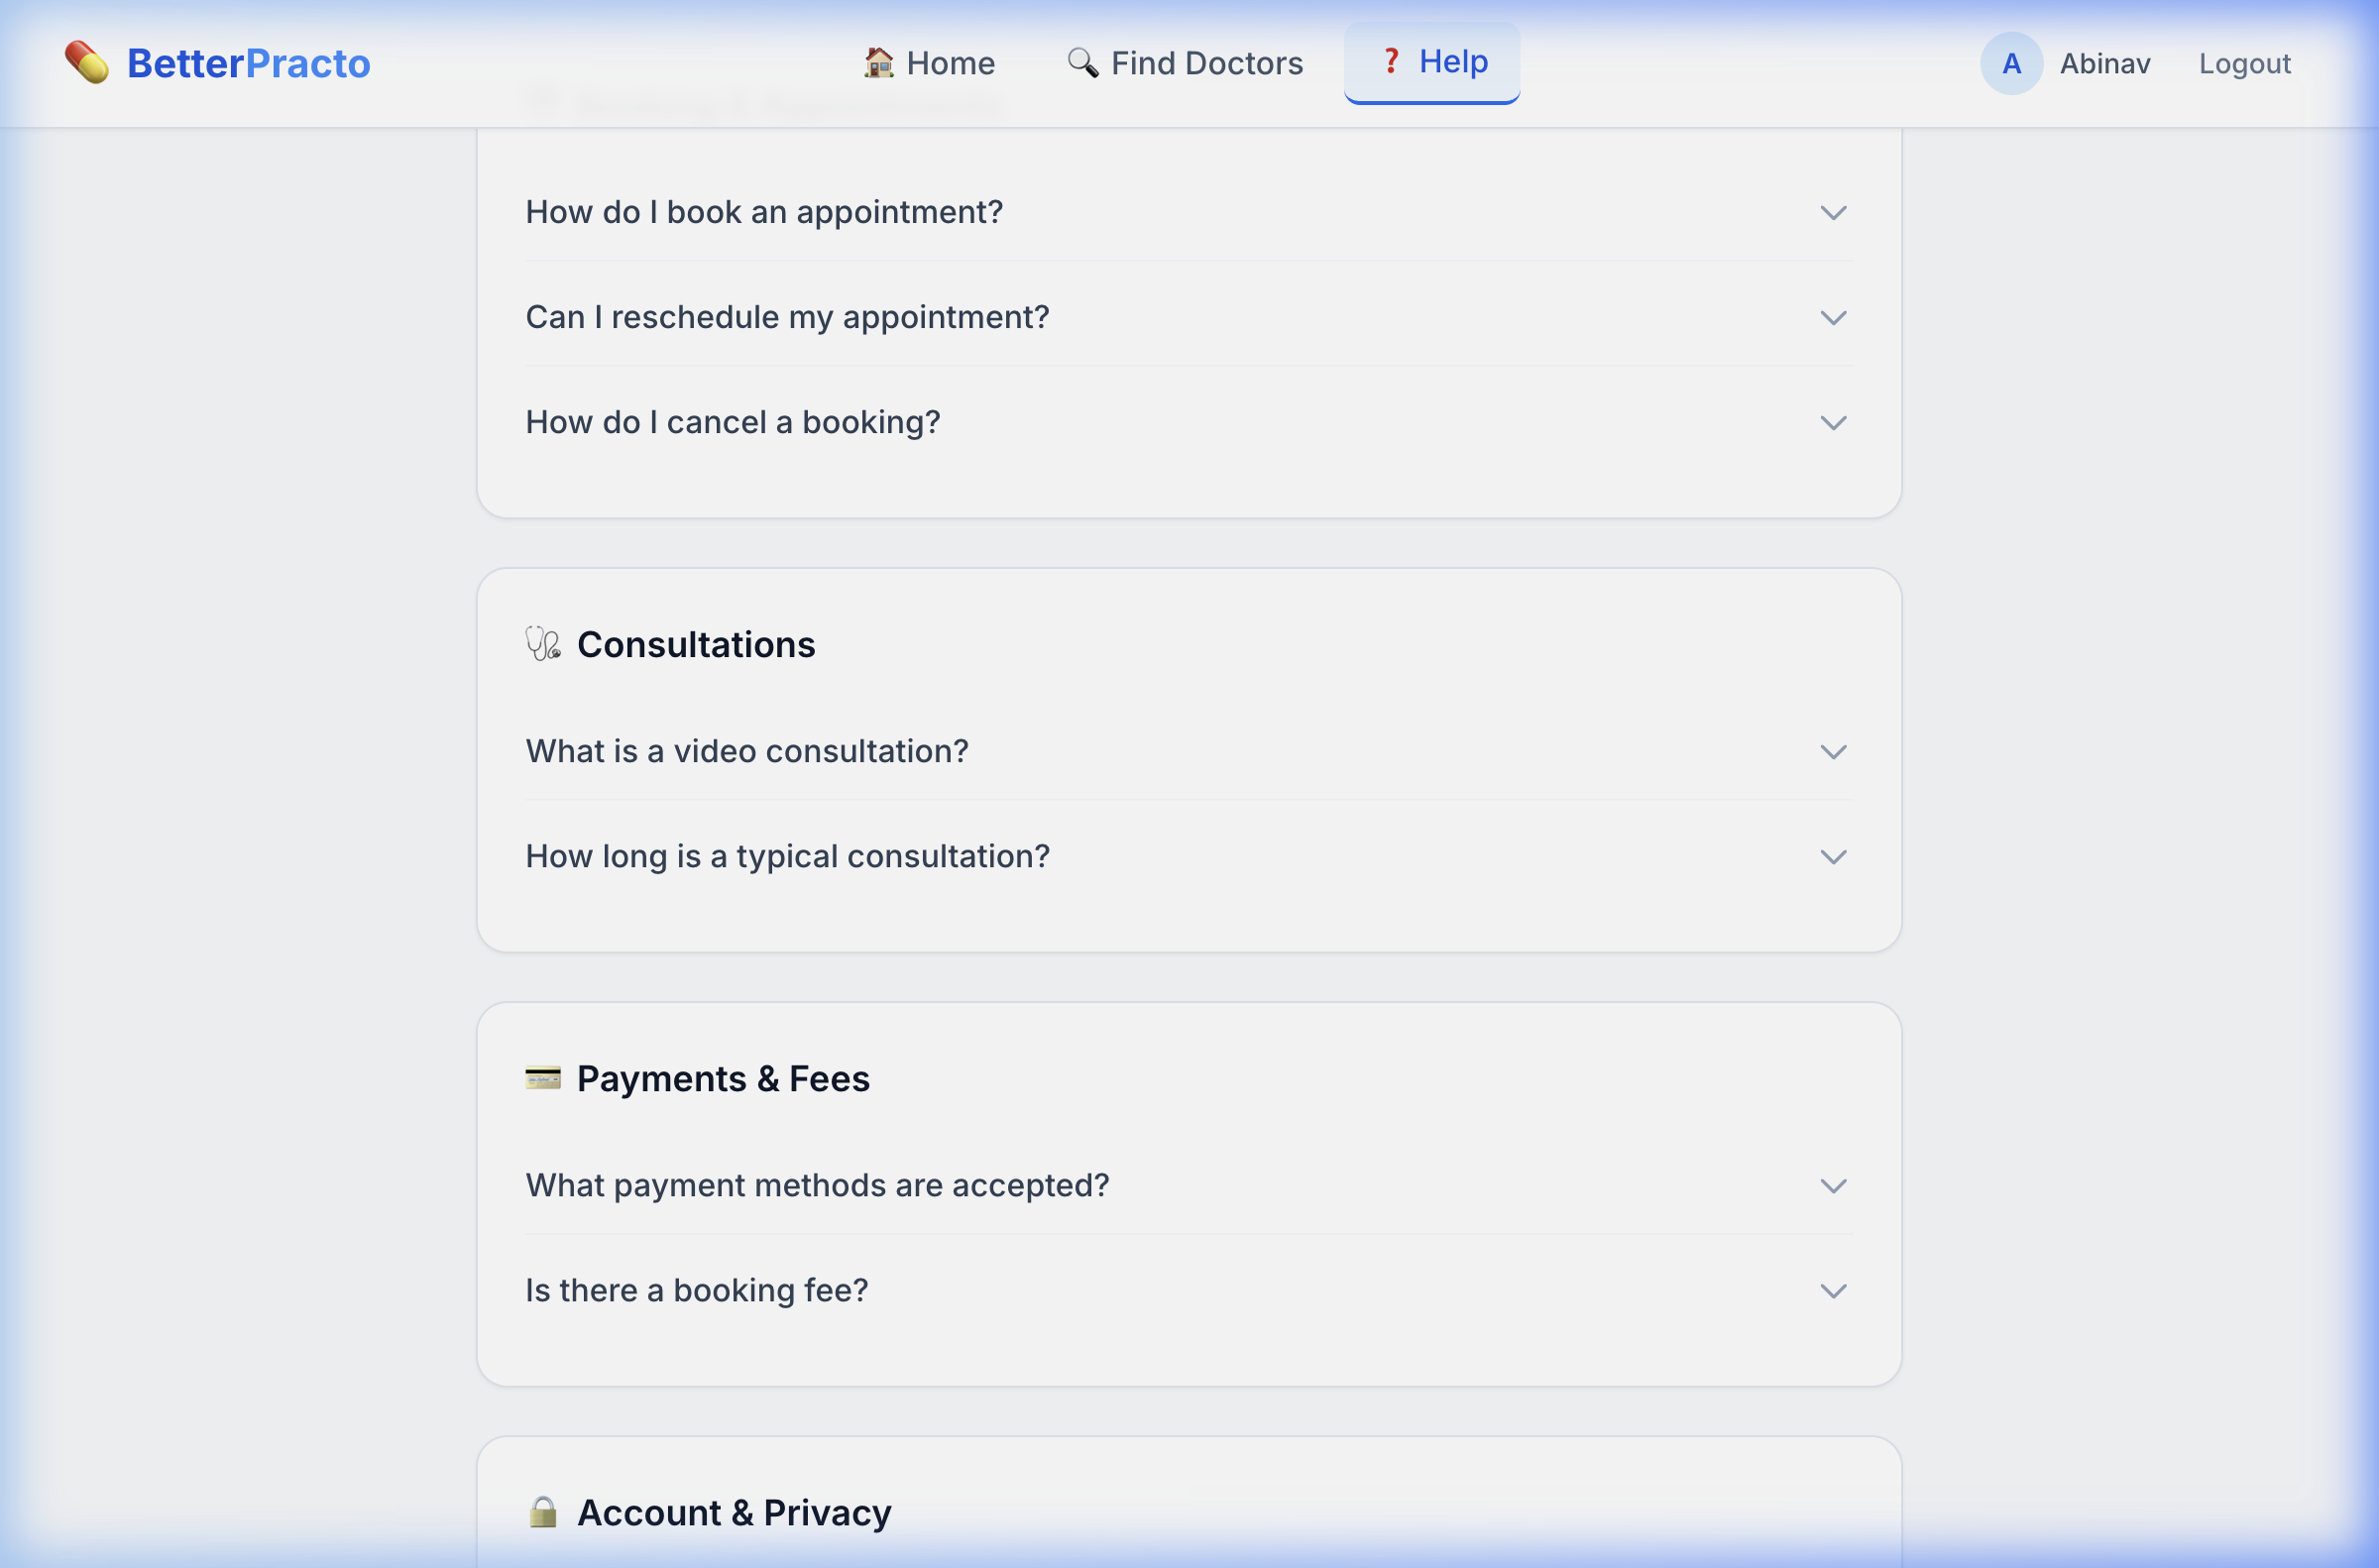
\includegraphics[width=0.8\textwidth]{our_help.png}
%     \caption{Better Practo --- In-app searchable FAQ, categorized by task}
% \end{figure}

\newpage

% ----------------------------------------------------------------
\subsection{V7: Small Text in Secondary Areas}

\begin{violationbox}
Practo uses small text (below 14px) in footer links, secondary labels, and card metadata, reducing readability, especially for older or visually impaired users.
\end{violationbox}

\begin{hcibox}{Accessibility, Observability (Robustness sub-principle)}
\textbf{Accessibility} standards recommend a minimum of 16px for body text and 14px for secondary text. \textbf{Observability} (Robustness sub-principle from Lecture 4) requires that users can perceive all relevant information --- small text undermines this.
\end{hcibox}

\begin{solutionbox}
Our entire app enforces a \textbf{minimum 14px font size}. Body text is 16px, labels are 14px, and no text goes below this threshold. We use the Inter font family for optimal readability. Proper color contrast ratios are maintained throughout.
\end{solutionbox}

\newpage

% ----------------------------------------------------------------
\subsection{V10: Important Content Not Left-Loaded}

\begin{violationbox}
On several Practo pages, important actions and information are placed on the right side of the screen (e.g., the ``Book Clinic Visit'' CTA on doctor profiles, map sidebar on search results), competing with or overshadowing the primary content path.
\end{violationbox}

\begin{hcibox}{Horizontal Attention Locus (69\% Left), F-Pattern (Lecture 6), Above the Fold}
Research shows \textbf{69\% of viewing time} is spent on the left half of the screen. The \textbf{F-Pattern} (Lecture 6) describes how users scan: across the top, then down the left side. \textbf{Above the Fold} --- 80\% of viewing time is spent above the fold.
\end{hcibox}

\begin{solutionbox}
All our pages follow the \textbf{F-Pattern}: primary content and actions are left-aligned. On the doctor profile, the main info occupies 2/3 of the width (left), with the booking CTA card on the right 1/3. On the home page, the search bar and hero cards are centered/left-loaded. Key information always appears above the fold.
\end{solutionbox}

\newpage

% ----------------------------------------------------------------
\subsection{V11: Reset Buttons on Forms}

\begin{violationbox}
Traditional form patterns often include a ``Reset'' or ``Clear All'' button alongside ``Submit''. This can accidentally destroy user input, causing frustration and data loss.
\end{violationbox}

\begin{hcibox}{Reset Must Die (Lecture 6), Shneiderman \#5 (Easy Reversal), Asimov's 1st Law (Do No Harm)}
The \textbf{Reset Must Die} case study (Lecture 6) argues that reset buttons are destructive and almost never what users want. \textbf{Shneiderman \#5} says reversal should be easy and granular, not all-or-nothing. \textbf{Asimov's 1st Law} --- the system should not harm the user (data loss = harm).
\end{hcibox}

\begin{solutionbox}
Our forms have \textbf{no reset button} anywhere. Instead:
\begin{itemize}[leftmargin=*]
    \item Each input field has an individual \textbf{clear button ($\times$)} to remove that specific field
    \item Users can go back to previous steps via ``$\leftarrow$ Change Slot'' (granular reversal)
    \item Form data is preserved when navigating between steps
\end{itemize}
\end{solutionbox}

\newpage

% ================================================================
\section{Complete HCI Concept Coverage}

The table below maps \textbf{every HCI concept from Lectures 1--8} to where it is applied in our design:

\begin{table}[H]
\centering
\small
\renewcommand{\arraystretch}{1.3}
\begin{tabularx}{\textwidth}{|l|l|X|}
\hline
\textbf{Lecture} & \textbf{Concept} & \textbf{Where Applied} \\
\hline
L1--2 & Affordance, Visibility & Buttons look clickable, inputs look typeable \\
L1--2 & Mental Models, Jakob's Law & Familiar health-app layout (top nav, search, cards) \\
\hline
L3 & Shneiderman \#1: Consistency & Uniform colors, spacing, components \\
L3 & Shneiderman \#3: Feedback & Loaders, progress bars, toasts \\
L3 & Shneiderman \#4: Closure & Booking confirmation with success animation \\
L3 & Shneiderman \#5: Easy Reversal & Back buttons, undo, individual field clear \\
L3 & Shneiderman \#8: Reduce STM & $\leq$5 nav items, chunked forms \\
\hline
L3 & Nielsen \#1: Visibility & Active nav, loaders, progress bar \\
L3 & Nielsen \#5: Error Prevention & Form validation, confirmation dialogs \\
L3 & Nielsen \#6: Recognition > Recall & Doctor photos, specialty icons \\
L3 & Nielsen \#8: Aesthetic Minimalism & Clean cards, whitespace \\
L3 & Nielsen \#9: Error Recovery & Plain-language error messages \\
L3 & Nielsen \#10: Help \& Docs & In-app FAQ, searchable \\
\hline
L3 & Norman: Constraints & Disabled past dates, unavailable slots greyed \\
L3 & Norman: Mapping & $\leftarrow$ back, $\rightarrow$ next \\
\hline
L4 & Learnability: Predictability & Consistent layout across pages \\
L4 & Learnability: Synthesizability & Breadcrumbs, step indicators \\
L4 & Learnability: Familiarity & Icons match real-world meanings \\
L4 & Flexibility: Substitutivity & Search by text OR browse by category \\
L4 & Robustness: Observability & System state always visible \\
L4 & Robustness: Recoverability & Undo/cancel at every step \\
L4 & Fitts's Law & Large CTAs, small destructive buttons \\
\hline
L5 & Password Masking & Show/hide toggle (V9) \\
L5 & Horizontal Attention & Key content left-aligned (V10) \\
\hline
L6 & F-Pattern, Above Fold & Important info top-left, above fold \\
L6 & Alphabetical Must Die & Default sort: relevance (V12) \\
L6 & Reset Must Die & No reset button (V11) \\
L6 & Headline Usability & Front-loaded, concise headings in FAQ \\
\hline
L7--8 & Miller's 7$\pm$2 & $\leq$5 nav items, $\leq$7 footer items/group \\
L7--8 & Serial Position Effect & Important items first/last in nav \\
L7--8 & Pareto / Vital Few & 4 hero cards = critical 20\% features \\
L7--8 & Zipf's / Least Effort & Most-used features = fewest clicks \\
L7--8 & Power Law of Practice & Consistent patterns for transfer \\
L7--8 & Asimov's 1st (No Harm) & Confirm destructive actions, autosave \\
L7--8 & Asimov's 2nd (No Waste) & Auto-detect location (V13) \\
L7--8 & Asimov's 3rd (Humane) & Respect cognitive limits \\
L7--8 & Tesler's Law & System absorbs complexity \\
\hline
\end{tabularx}
\caption{Complete HCI concept mapping from Lectures 1--8}
\end{table}

\newpage

% ================================================================
\section{Summary of Violations \& Solutions}

\begin{table}[H]
\centering
\small
\renewcommand{\arraystretch}{1.3}
\begin{tabularx}{\textwidth}{|c|X|X|X|}
\hline
\textbf{V\#} & \textbf{Practo Violation} & \textbf{HCI Principles} & \textbf{Our Fix} \\
\hline
V1 & Footer with 50+ links & Miller's 7$\pm$2, Hick's Law, Tesler's & Collapsible footer, $\leq$7 items/group \\
\hline
V2 & Dual search bar & Tesler's, Zipf's, Asimov's 2nd & Unified search + auto-location \\
\hline
V3 & Cluttered doctor cards & Inverted Pyramid, Nielsen \#8 & Progressive disclosure \\
\hline
V5 & Weak booking feedback & Closure, Shneiderman \#3/\#4 & Progress bar + success animation \\
\hline
V6 & No contextual help & Nielsen \#10, Shneiderman \#8 & Searchable in-app FAQ \\
\hline
V7 & Small secondary text & Accessibility, Observability & Min 14px, proper contrast \\
\hline
V8 & Inconsistent active nav & Nielsen \#1, Shneiderman \#1 & Consistent active indicators \\
\hline
V9 & Password fully masked & Password Masking case study & Show/hide toggle \\
\hline
V10 & Content not left-loaded & Horizontal Attention, F-Pattern & Left-aligned key content \\
\hline
V11 & Reset buttons on forms & Reset Must Die, Shneiderman \#5 & No reset; individual clear \\
\hline
V12 & Alphabetical sort default & Alphabetical Must Die & Default: relevance/rating \\
\hline
V13 & Forced city selection & Asimov's 2nd, Zipf's & Auto-detect location \\
\hline
V14 & No booking progress bar & Closure, Synthesizability & 3-step indicator with labels \\
\hline
\end{tabularx}
\caption{Summary of all 14 violations and solutions}
\end{table}

% ================================================================
\section{Additional Links}

\begin{itemize}[leftmargin=*]
    \item \textbf{Working Prototype}: Run \texttt{npm run dev} in the project directory
    \item \textbf{Source Code}: \url{https://github.com/R-Abinav/hci-mid-design-activity}
    \item \textbf{Tech Stack}: React + Tailwind CSS (Vite build system)
    \item \textbf{Demo Credentials}: \texttt{user@betterpracto.com} / \texttt{password123}
\end{itemize}

\end{document}
